\documentclass[11pt,a4paper,english]{article}
\usepackage[T1]{fontenc}
\usepackage[utf8]{inputenc}
\usepackage{babel}
\usepackage{blindtext}
\usepackage{hyperref}
\usepackage{graphicx}
\usepackage{float}

\setlength\fboxsep{0.25cm}
\setlength\fboxrule{0pt}


\title{Correlation of Forum Activity and real world events based on a social network dataset}
\author{%
  Cedric Waldburger\thanks{data provided by ASmallWorld Holding, New York}\\
  \small Department of Electrical Engineering\\
  \small ETH Zurich \\
  \small\texttt{ctwaldburger@student.ust.hk}
  \and
  Christoffer Hirsimaa\\
  \small Department of Computer Science\\
  \small KTH Stockholm\\
  \small\texttt{cahirsimaa@stu.ust.hk}
}

\begin{document}
  \maketitle

  \begin{abstract}
    We've used the data from invitation-only network ASmallWorld.net to analyze correlations of forum activity and real life events.
  \end{abstract}
  \newpage

  \tableofcontents\newpage

	\section{Goal}
		\subsection{About ASmallWorld}
			ASmallWorld.net (ASW) is a unique social media combining a by-invitation-only social network with a content delivery platform targeting the "upper end" of the social media market. Founded in 2004 even before facebook became popular, ASW stayed the market leader in this segment. As An integrated media company, ASW is an ideal match for advertisers seeking to target the world's tastemakers and develop heightened mindshare with this sophisticated and influential group.
			\\Some of the site's features are: \begin{itemize}
				\item a lifestyle and travel magazine called ASmallMagazine
				\item an eBay-like platform where members trade everything from computers to Houses and Yachts
				\item a GeoLocator, where member log their trips, ask for sightseeing advice and find selected services for every destination in the Travel Guides
				\item a Forum where people seek business advice, look for like-minded members all over the globe or discuss current happenings
				\item many more, less used features
			\end{itemize}
			With ASW existing before many of the other web 2.0 sites, it's forum was and is heavily used also to discuss politics and current news. Rumors say, that in 2004 and 2005, ASW members would be faster at posting news to the site's forum than journalists had their news on their respective news websites and ASW functioned as an 'information hub'.
			\\ Based on this rumor, we decided to see whether it is possible to find correlations between the forum's activity and the real world happenings.
			
		\subsection{Our objective}
			In order to find out, how correlated ASW's forum activity and real life news are, we are building a tool to visualize forum activity over a certain time span using the Google Maps API.
			\\ We'll use the visualized activity to \begin{itemize}
				\item have a look at the word wide activity to see if there is a substantial part of the world wide activity is coming from the particular area of the real life's event
				\item zoom in on that particular region and compare the time span of the real life's event with the weeks before to see if activity increased
			\end{itemize}
			We'll then try to conclude where and when the activity on the forum increased due to real life events.
			
		\subsection{Facts \& Figures}
			\begin{itemize}
				\item \bf Total number of records: \rm 254 622
				\item \bf First record: \rm June 7, 2004
				\item \bf Last record: \rm February 2, 2011
				\item \bf database size and type: \rm 19.5 MB, sqlite3
				\item \bf geography: \rm ASW's user base is concentrated in Europe and the east and west coast of the United States (with a main concentration in New York/Boston and Los Angeles/San Francisco)
			\end{itemize}
			 		
	\section{Approach}
		\subsection{Getting the Data}
		ASW uses a SQL-based database to store their data. We were granted to access all their data from mid 2004 until early 2010. Using scripting languages, we converted the database dump into a sqlite database that we could afterwards use locally and online without setting up a database server. The database contained one table with each record containing this information: 
		\\ id, post\_id, creation\_date, member\_id, member\_city, lng (langitude), lat (latitude) 
		
		\subsection{Building the Visualizer}
		We used the Google Maps API in javascript to put out circles on a map. We basically put out two date pickers so you could define a time period to visualize in a specified speed. By starting the animation it starts to iterate over each date and for each date make an asynchronized AJAX call to retrieve the posts from the server. The iteration is done by setInterval method so that the browser don't freeze during visualisation. Posts are iterated over to create new circles on the map or increase the size and color intensity. The size and opacity are calculated according to the following formulas \ref{rad} and \ref{opa} for each circle.

		\begin{equation} \label{rad}
			 radius = 20000*log(10* number Of Posts)
		\end{equation}
		\begin{equation} \label{opa}
			 opacity = 0.2*log( number Of Posts )
		\end{equation}

		These formulas were found by trail and error and they resulted in very detailed images.
		
		\subsection{Setting up the Experiment}
		In order to test our hypothesis that real life events and the forum activity are correlated, we decided to only look at the years with a full dataset (2005-2008) and for each year to select 3 events:
		\begin{itemize}
			\item an event that was present in public newspapers for approximately 1 week
			\item an event that was present for approximately 2 weeks
			\item an event that was discussed in the news for a month or longer
		\end{itemize}
		We selected the events based on \url{http://moldova.org} and we referred to the particular article at the beginning of each year. Then we compared the activity on relevant locations before the event and during it's public presence. To make the comparison fair the duration of visualizing before and during events is the same.
		\\ We chose events from the following geographical locations (some events are affecting more than one location):
		\begin{itemize}
			\item 9 events affecting Europe
			\item 4 events affecting the US
			\item 6 events affecting Asia
			\item 1 events affecting South America
		\end{itemize}

 \newpage

	\section{Experiments - News Events}
			\subsection{2005}
			\href{http://politicom.moldova.org/news/10-most-important-world-events-of-2005-7712-eng.html}{Top10 Events in 2005 on moldova.org}
				\begin{itemize}
				\item \bf Death of Pope John Paul II\rm
					\\ The death of Pope John Paul II marked the end of an era in the life of the Roman-Catholic Church and modern history. 
					\\\\ \bf time span: \rm April 2 - April 9
					\\ \bf geographical area: \rm Vatican
					\\ \bf total number of threads: \rm 347

					\begin{figure}[H]
						\vspace{-10pt}	
						\begin{center}
							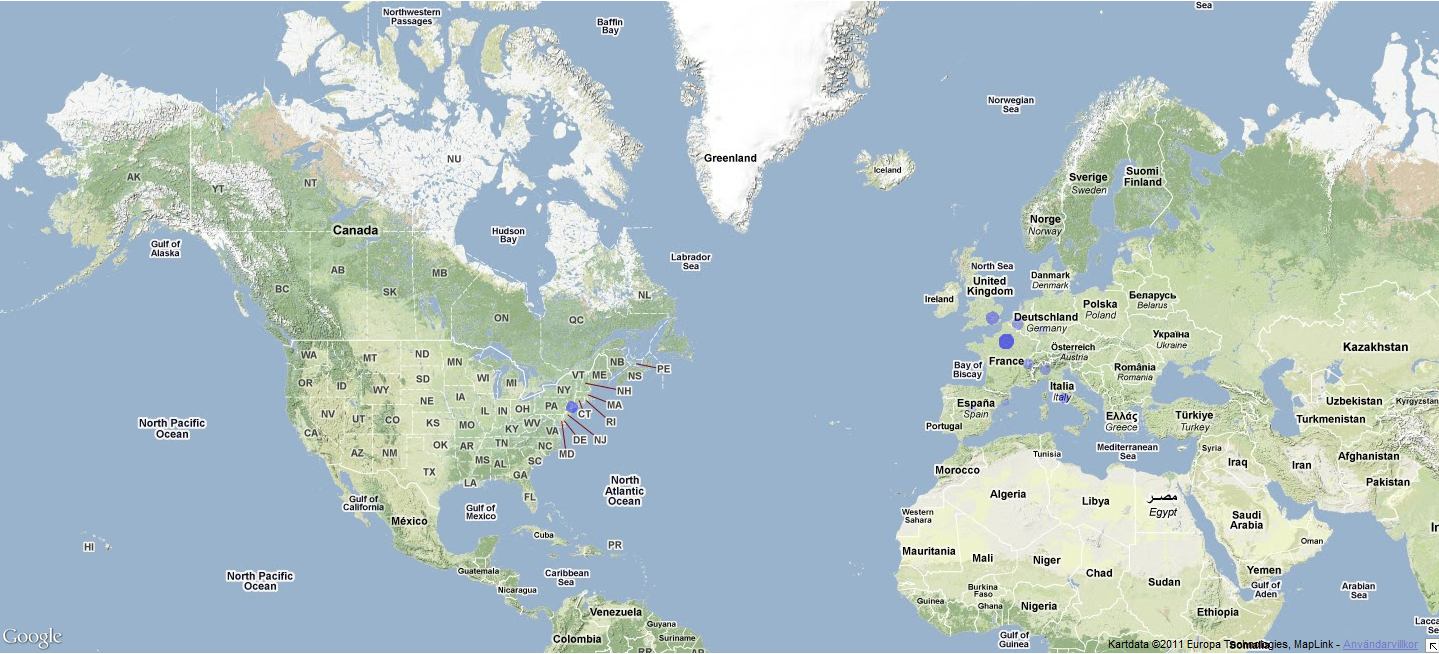
\includegraphics[width=130mm]{img/pre-pope}
						\end{center}
						\vspace{-13pt}
					\end{figure}
					\begin{figure}[H]
						\vspace{-10pt}
  						\begin{center}
							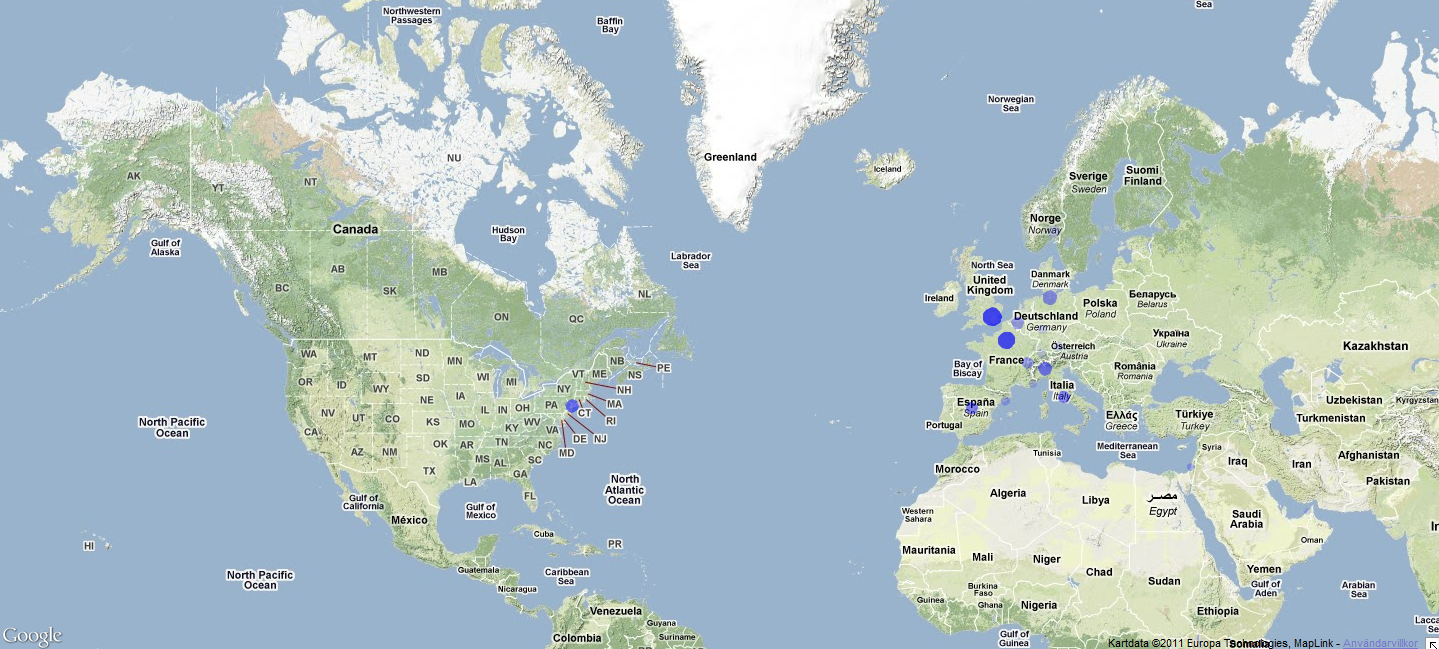
\includegraphics[width=130mm]{img/post-pope}
						\end{center}
						\vspace{-13pt}
					\end{figure}
						
					\bf interpretation: \rm correlated
					\\ Compared the the week before, we saw an increased activity in many european countries including the UK, Denmark, the South of France, Spain, Switzerland and Italy. Even though the Death of Pope John Paul II is definitely an event with worldwide attention, it is reasonable that it was most discussed around central europe from the the Pope was originally from (Poland). We expected to see more activity in Italy, close to the Vatican, however we can definitely say that there's a strong correlation between the Pope's death and activity on ASW in central Europe.
						


				\item \bf Terrorist act in London \rm
					\\ A terrorist act in London overshadowed the G8 summit in Gleneagles, Scotland, and spoiled Britons' joy over London's election as the host city for the 2012 Olympics. Four explosive devices went off in the underground and a bus, leaving 50 people dead and about 700 injured.
					\\\\ \bf time span: \rm July 7 - July 21
					\\ \bf geographical area: \rm London, UK
					\\ \bf total number of threads: \rm 498
					\begin{figure}[H]
						\vspace{-10pt}
						\begin{center}
							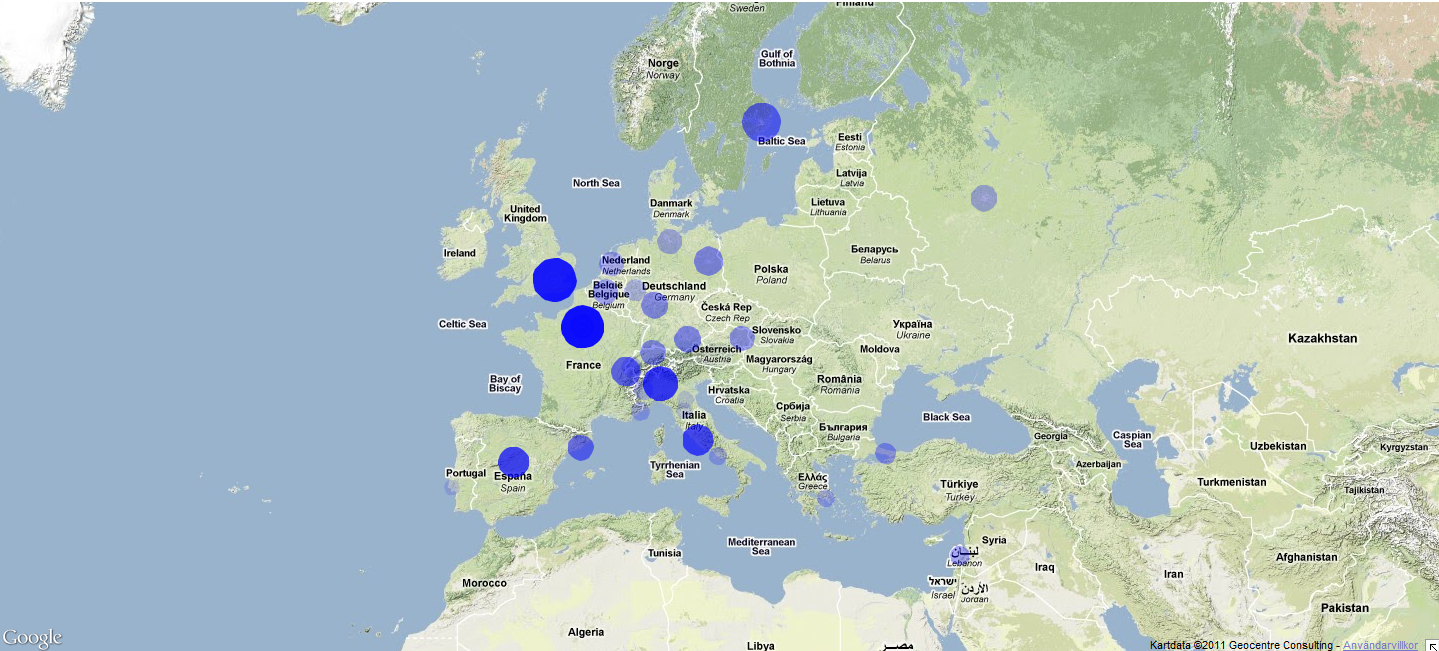
\includegraphics[width=130mm]{img/pre-london}
						\end{center}
						\vspace{-13pt}
					\end{figure}
					\begin{figure}[H]
						\vspace{-10pt}
  						\begin{center}
							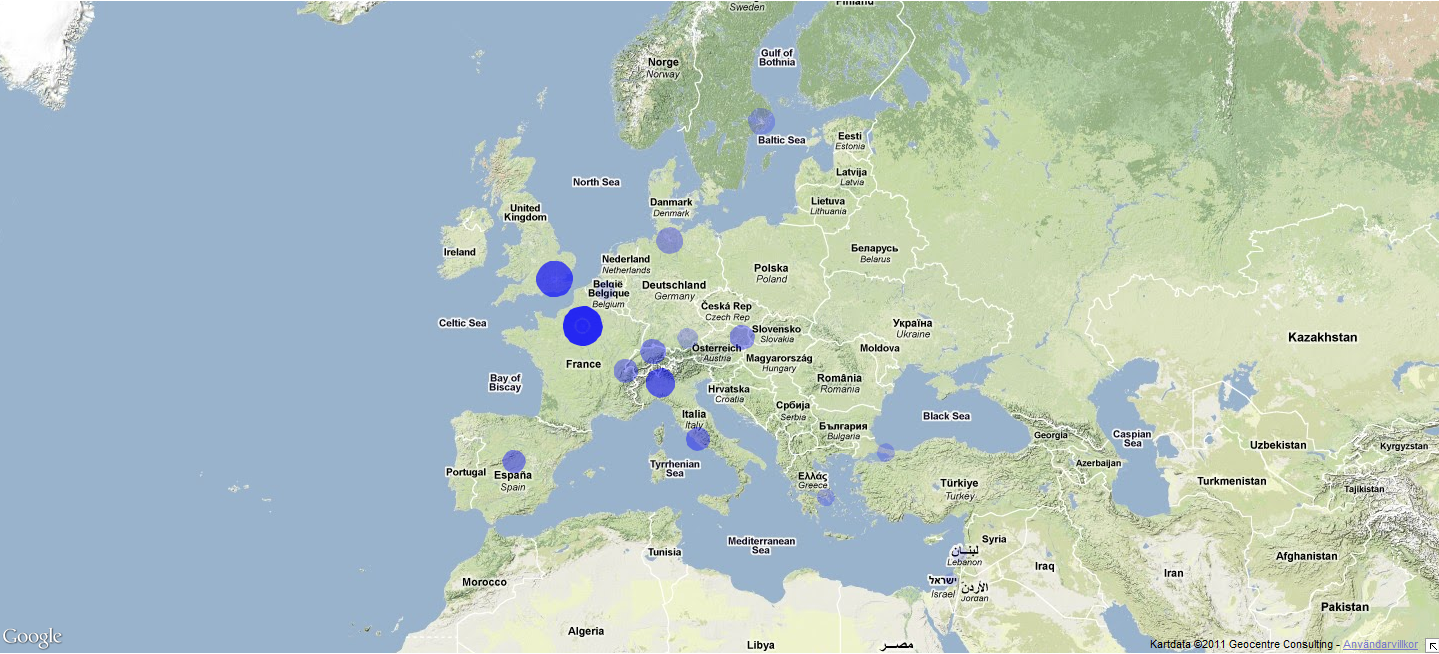
\includegraphics[width=130mm]{img/post-london}
						\end{center}					
						\vspace{-13pt}
					\end{figure}
					
					\bf interpretation: \rm correlated
					\\ On the first day of the event there's a massive amount of activity in Paris and London, which proofs that the event and the network activity are definitely correlated. During the week after the event there was more activity in central europe and also cities that usually show not much activity were opening forum threads in large numbers - this includes cities in the Netherlands, Belgium, all over Germany and even in Russia.

						
				\item \bf Hurricane Katrina \rm
					\\ Hurricane Katrina in the United States showed that the world's leading super power was unprepared to deal with the aftermath of the natural disaster. The hurricane destroyed the cradle of jazz, New Orleans. 
					\\\\ \bf time span: \rm August 23 - September 23
					\\ \bf geographical area: \rm USA
					\\ \bf total number of threads: \rm 4108
					\begin{figure}[H]
						\vspace{-10pt}
  							\begin{center}
								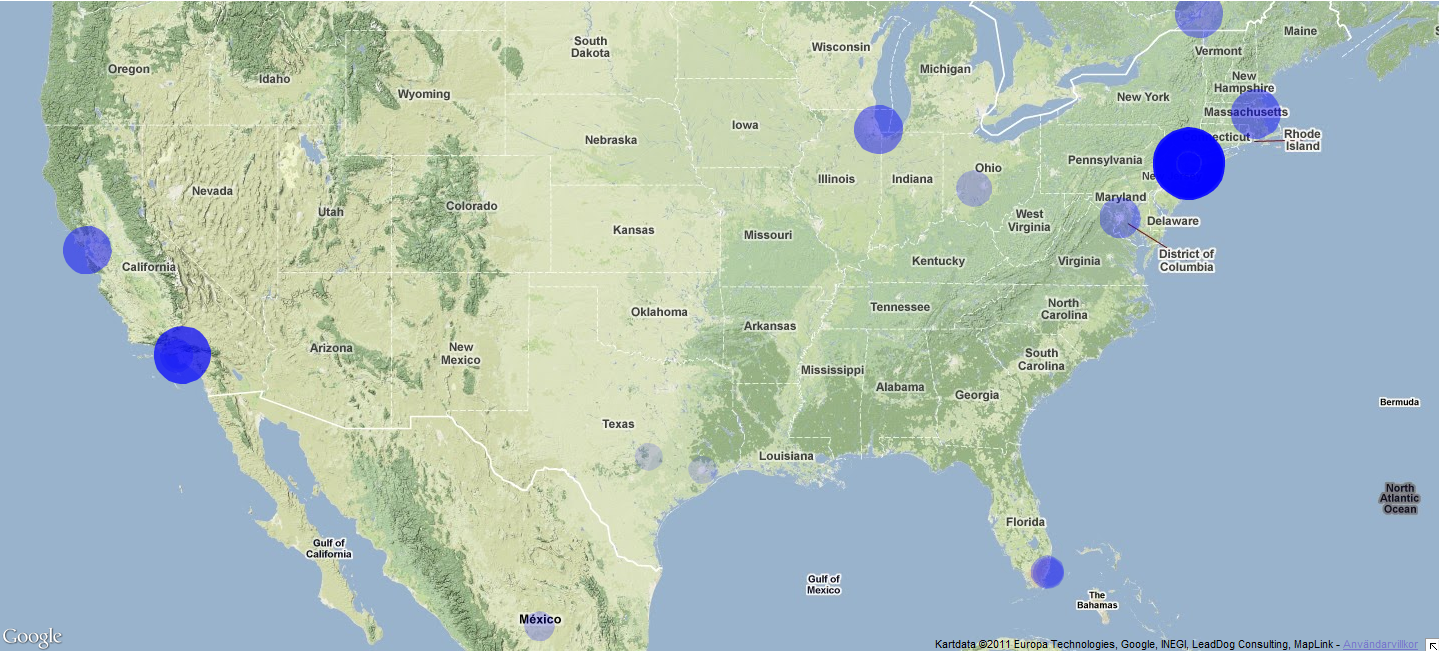
\includegraphics[width=130mm]{img/pre-katrina}
							\end{center}
							\vspace{-13pt}
					\end{figure}
					\begin{figure}[H]
						\vspace{-10pt}
						\begin{center}
							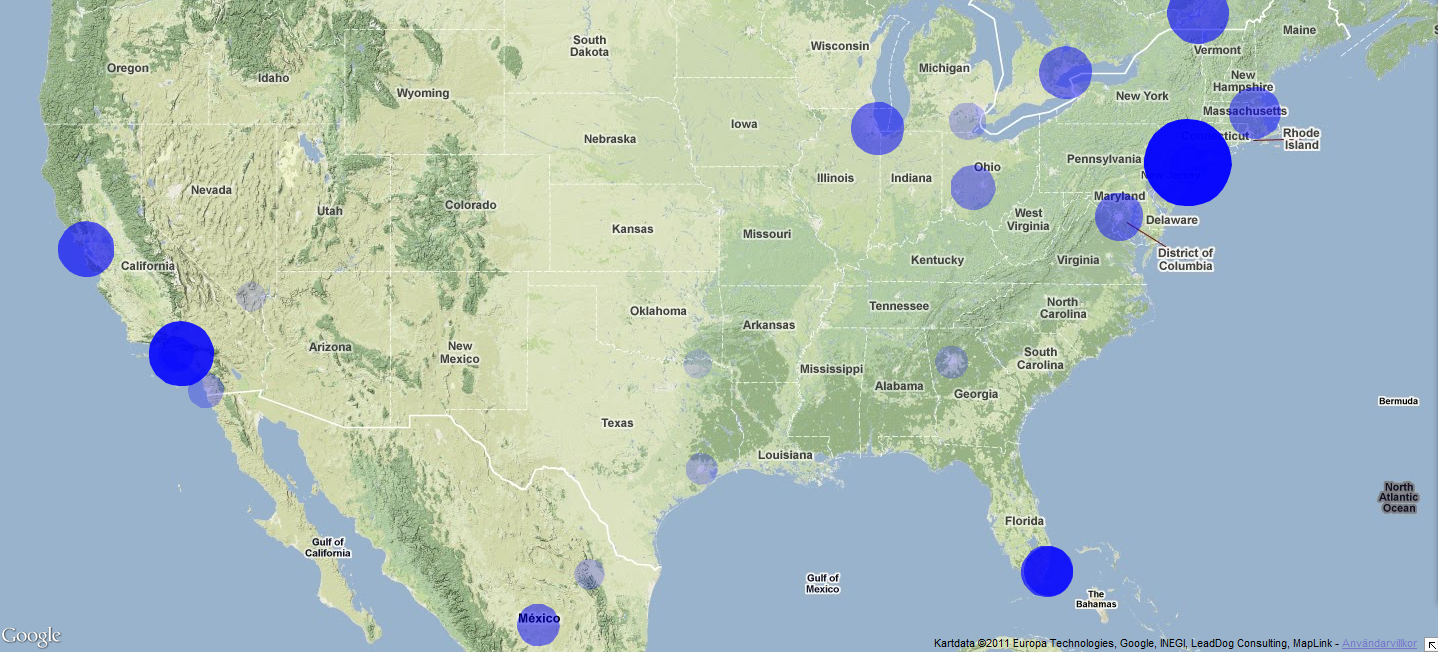
\includegraphics[width=130mm]{img/post-katrina}
						\end{center}					
						\vspace{-13pt}
					\end{figure}
					
					\bf interpretation: \rm correlated
					\\ The month after Hurricane Katrina, New York showed a lot more activity than usual (the bulb's size is logarithmic to the number of posts) and all over the US new circles popped up, also in areas where there's almost no activity otherwise. This is true for the northern and southern part and also for the east and West Coast. There's no activity in New Orleans which is probably due to a very small user base in that area.
					
					
												
				\end{itemize}
			
			\subsection{2006}
			\href{http://social.moldova.org/news/10-most-important-world-events-of-2006-217385-eng.html}{Top10 Events in 2006 on moldova.org}
				\begin{itemize}
					\item \bf Bird Flu \rm
						\\ People watched nervously as the infamous disease spread from Asia to Europe. But flu season died down before disaster struck. The human being was in a big danger, as a current H5N1 strain is a fast-mutating, highly pathogenic avian influenza virus (HPAI) found in multiple bird species.
						\\\\ \bf time span: \rm January 1 - January 14
						\\ \bf geographical area: \rm Asia
						\\ \bf total number of threads: \rm 25930
						\begin{figure}[H]
							\vspace{-13pt}
  							\begin{center}
								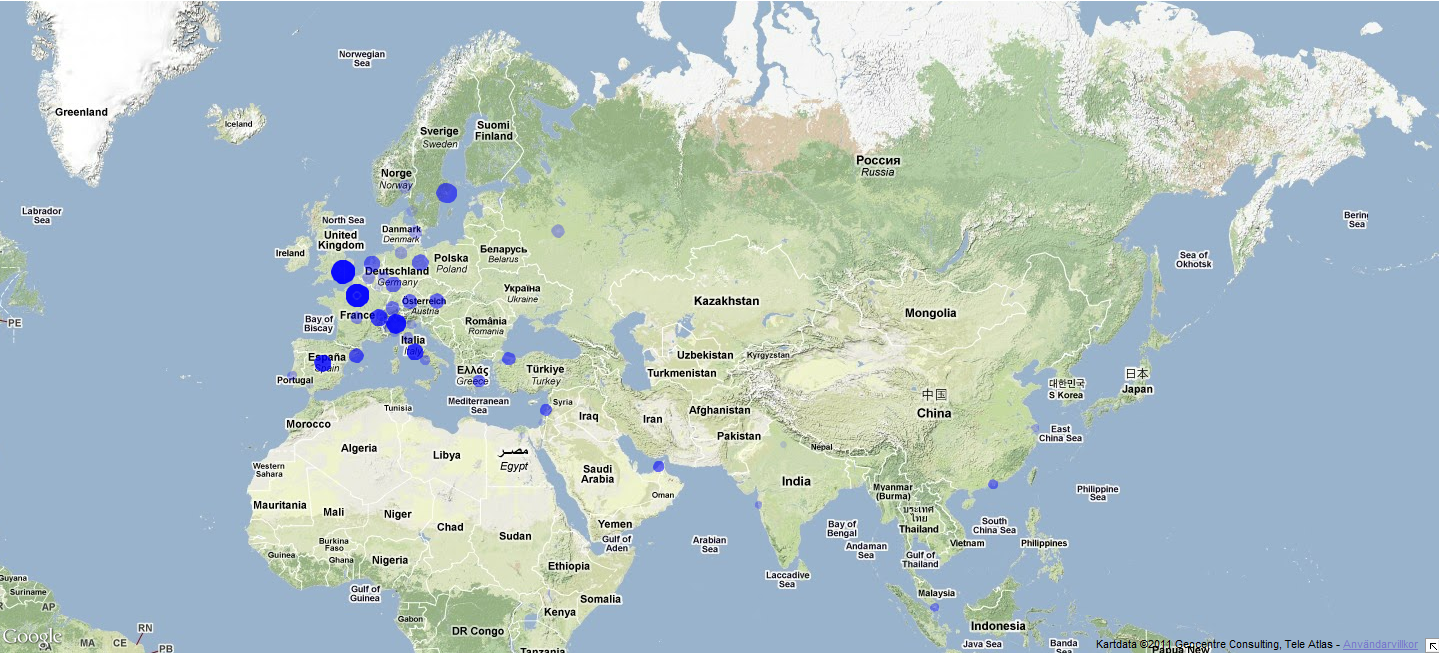
\includegraphics[width=130mm]{img/pre-birdflu}
							\end{center}
							\vspace{-13pt}
						\end{figure}
						\begin{figure}[H]
							\vspace{-13pt}
	  						\begin{center}
								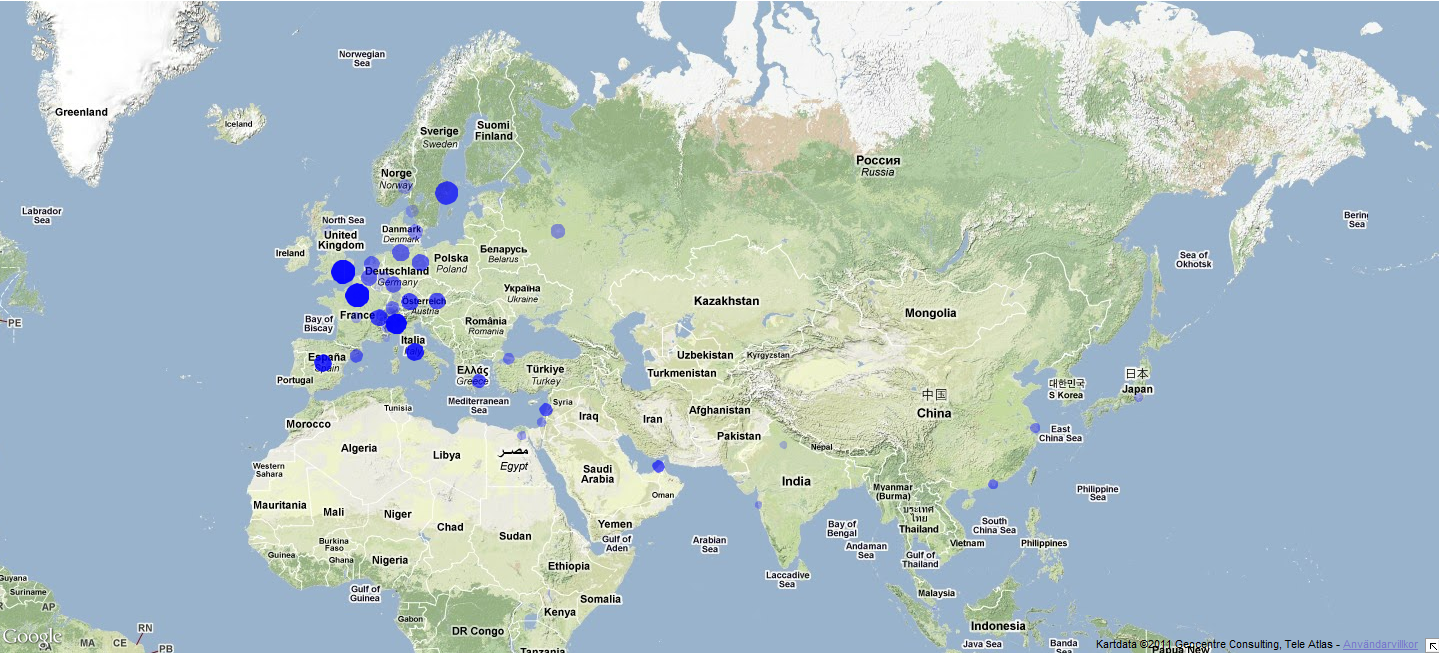
\includegraphics[width=130mm]{img/post-birdflu}
							\end{center}
							\vspace{-13pt}
						\end{figure}
						
						\bf interpretation: \rm not correlated
						\\ There's more activity in Greece, Portugal, Scandinavia, Egypt, Syria, Singapur and Shanghai. As for Europe this could be due to minor local activities in those countries and as for Asia there's not a big increase to normal activity and the network activity therefore was probably not correlated to the Bird Flu.
	
					
					\item \bf Soccer World Cup \rm
						\\ Italy wins the World Cup 5-3 vs. France.
						\\\\ \bf time span: \rm June 9 - July 9
						\\ \bf geographical area: \rm Central Europe (Cup held in Germany)
						\\ \bf total number of threads: \rm 4326
						
						\begin{figure}[H]
							\vspace{-13pt}
  						
  							\begin{center}
									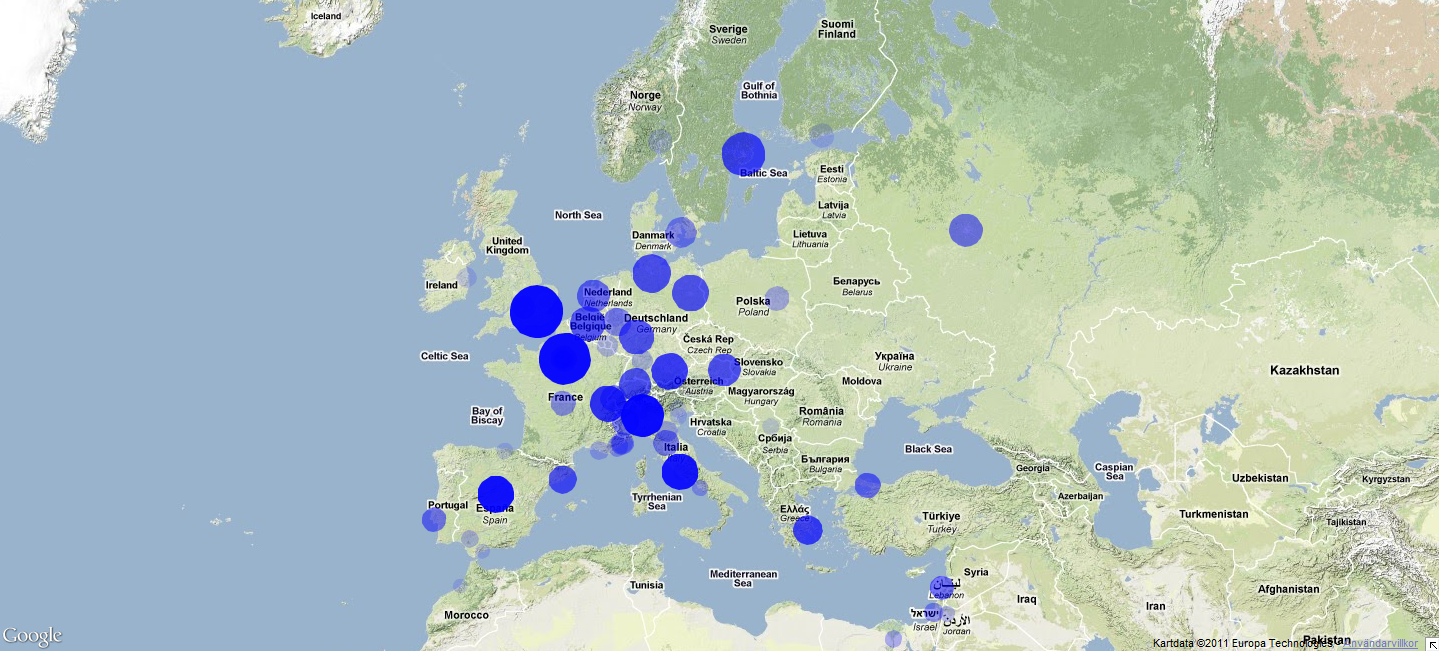
\includegraphics[width=130mm]{img/pre-wcfinal}
									\vspace{-13pt}
								\end{center}
						\end{figure}
						\begin{figure}[H]
							\vspace{-13pt}
	  						\begin{center}
									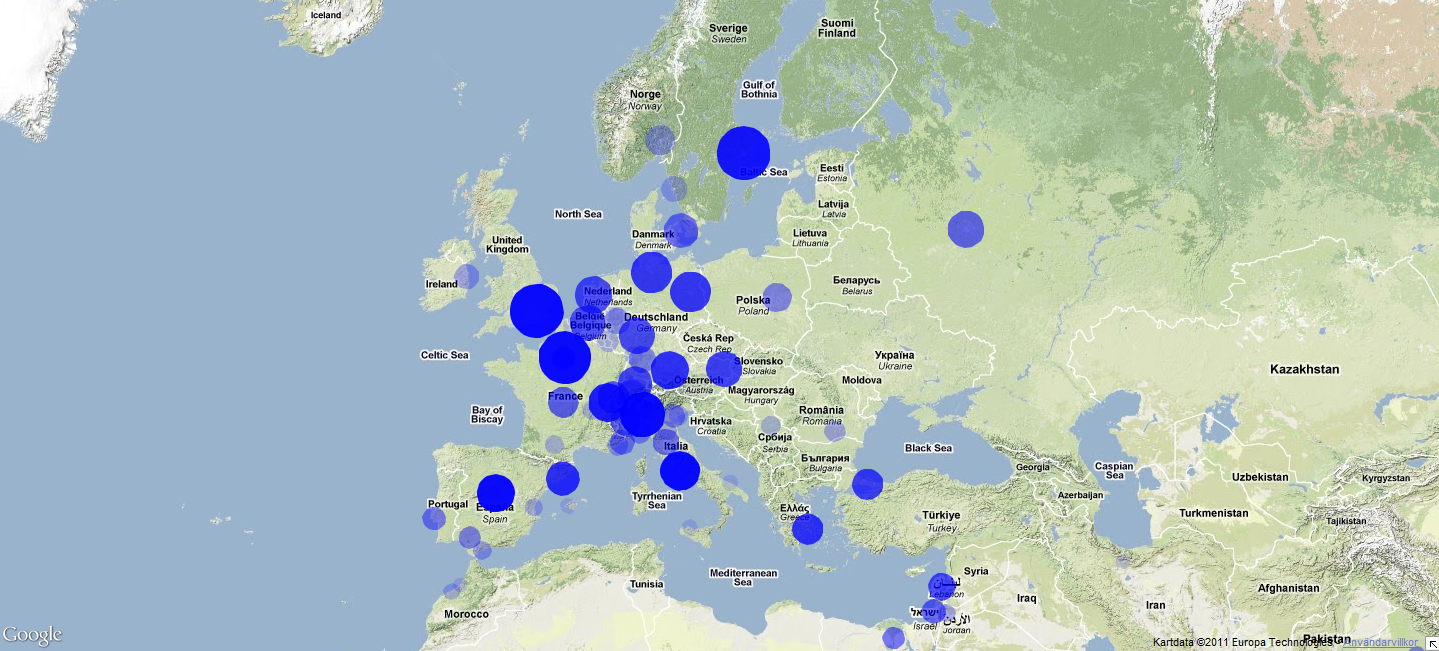
\includegraphics[width=130mm]{img/post-wcfinal}
							\end{center}
							\vspace{-13pt}
						\end{figure}							
						\bf interpretation: \rm correlated
						\\ Even the month before the world cup, there's a lot more activity in europe than usual. During the world cup almost every ASW member city was active in the forum. The existing circles got a bit bigger during this month and there's new activity in the north of Spain, South of France, all over Italy, Ireland, Scandinavia and many others. This month showed so much more activity in smaller and also bigger european cities compared to other months that it is very likely to be related to the World Cup.
						
						
					
					\item \bf Saddam Hussein sentenced to death \rm
						\\ Saddam Hussein sentenced to death by hanging by an Iraqi court. Earlier in this year he was charged with genocide by an Iraqi court for a campaign against Iraq's Kurdish population in 1988.
					\\\\ \bf time span: \rm November 5 - November 12
						\\ \bf geographical area: \rm Iraq
						\\ \bf total number of threads: \rm 1212
						\begin{figure}[H]
							\vspace{-13pt}
  							\begin{center}
								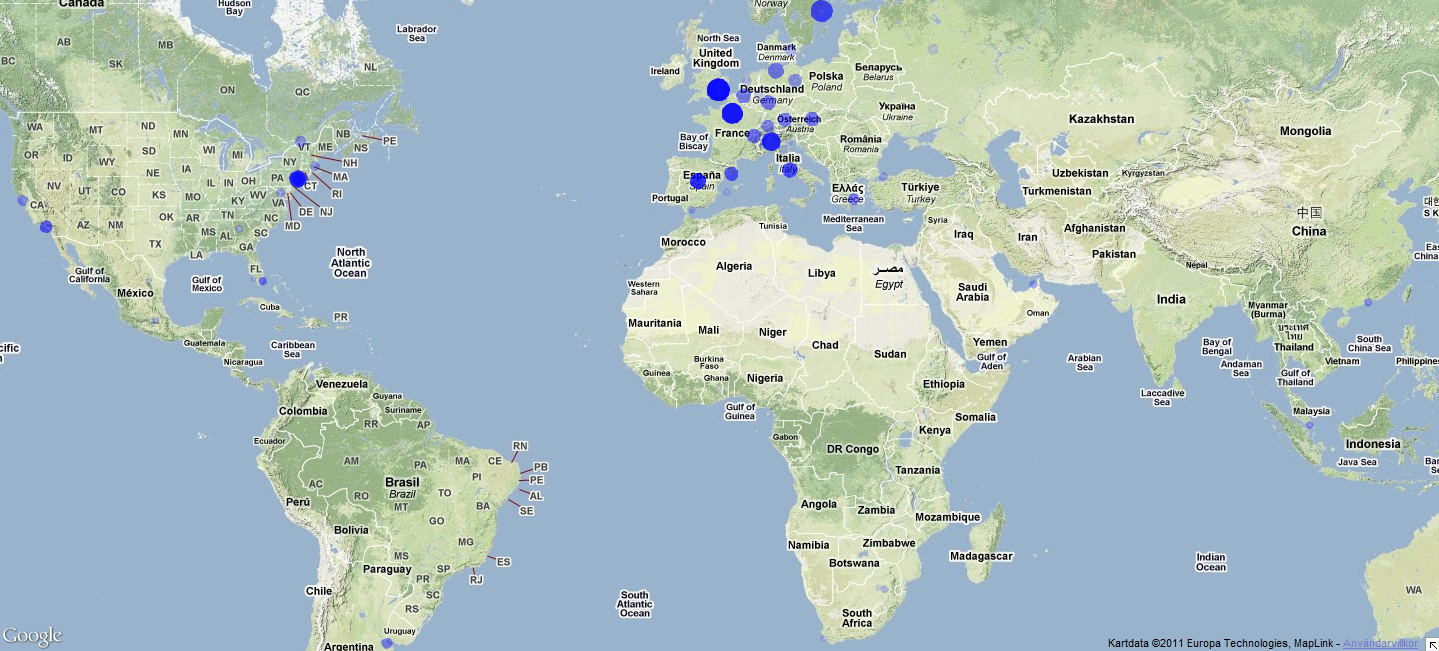
\includegraphics[width=130mm]{img/pre-saddam}
							\end{center}
							\vspace{-13pt}
						\end{figure}
						\begin{figure}[H]
							\vspace{-13pt}
  							\begin{center}
								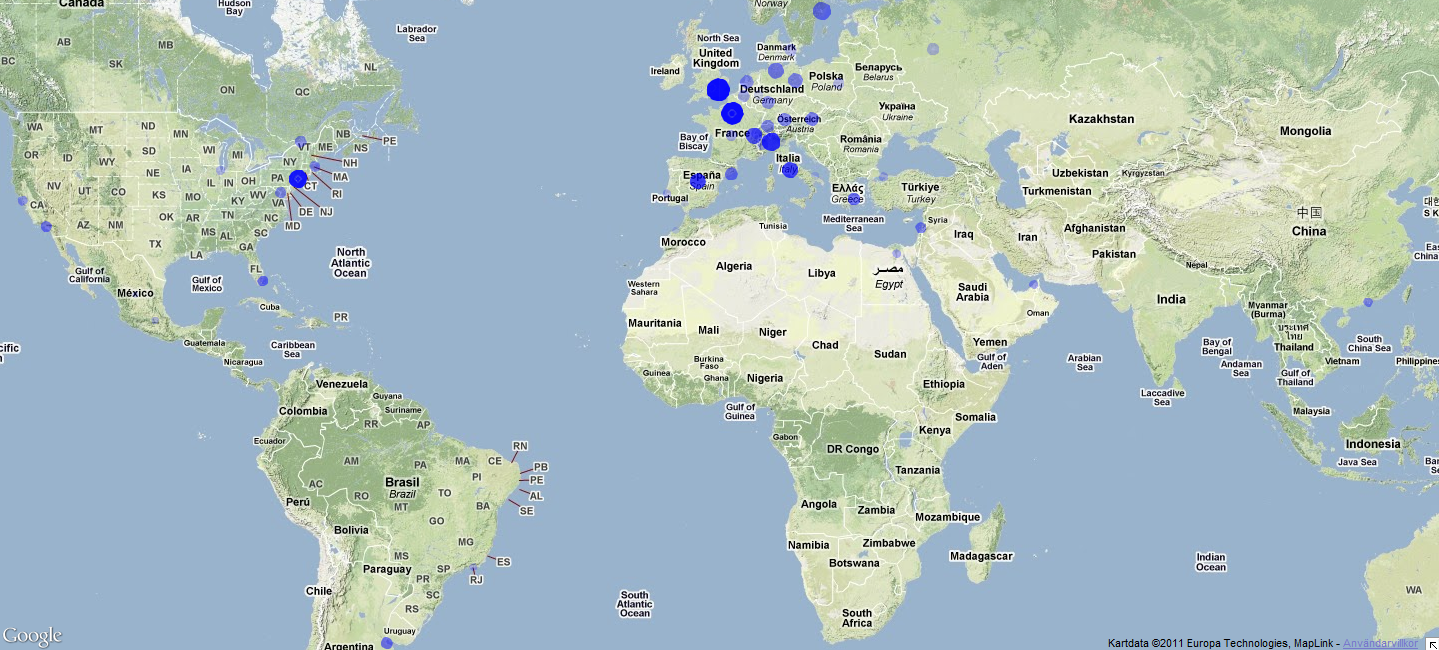
\includegraphics[width=130mm]{img/post-saddam}
							\end{center}
							\vspace{-13pt}
						\end{figure}	
						
					\bf interpretation: \rm not correlated
					\\ There are no posts at all from Iraq (maybe due to a limited number of users in this area) and also no drastic changes worlwide. In this case, forum activity is probably not related to Saddam Hussein's sentence to death.						
							
				\end{itemize}
			
			\subsection{2007}
			\href{http://social.moldova.org/news/10-most-important-world-events-of-2007-217388-eng.html}{Top10 Events in 2007 on moldova.org}
				\begin{itemize}
					\item \bf Gordon Brown becomes Prime Minister \rm
						\\ Gordon Brown replaces Tony Blair as the prime minister of Great Britain (June 27). "Let the work of change begin," said Brown in the day he was elected.
						\\\\ \bf time span: \rm June 27 - July 4
						\\ \bf geographical area: \rm UK
						\\ \bf total number of threads: \rm 2098
						\begin{figure}[H]
							\vspace{-13pt}
  							\begin{center}
								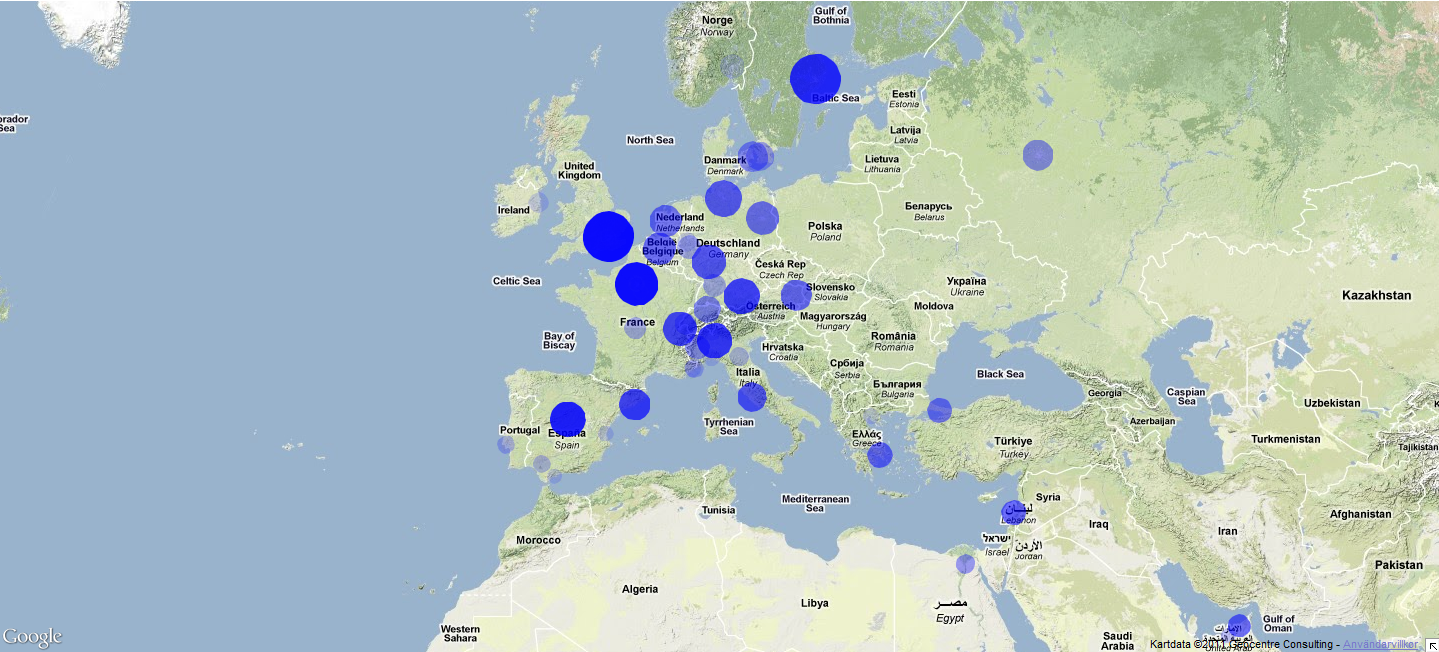
\includegraphics[width=130mm]{img/pre-gordon}
							\end{center}
							\vspace{-13pt}
						\end{figure}
						\begin{figure}[H]
							\vspace{-13pt}
	  						\begin{center}
									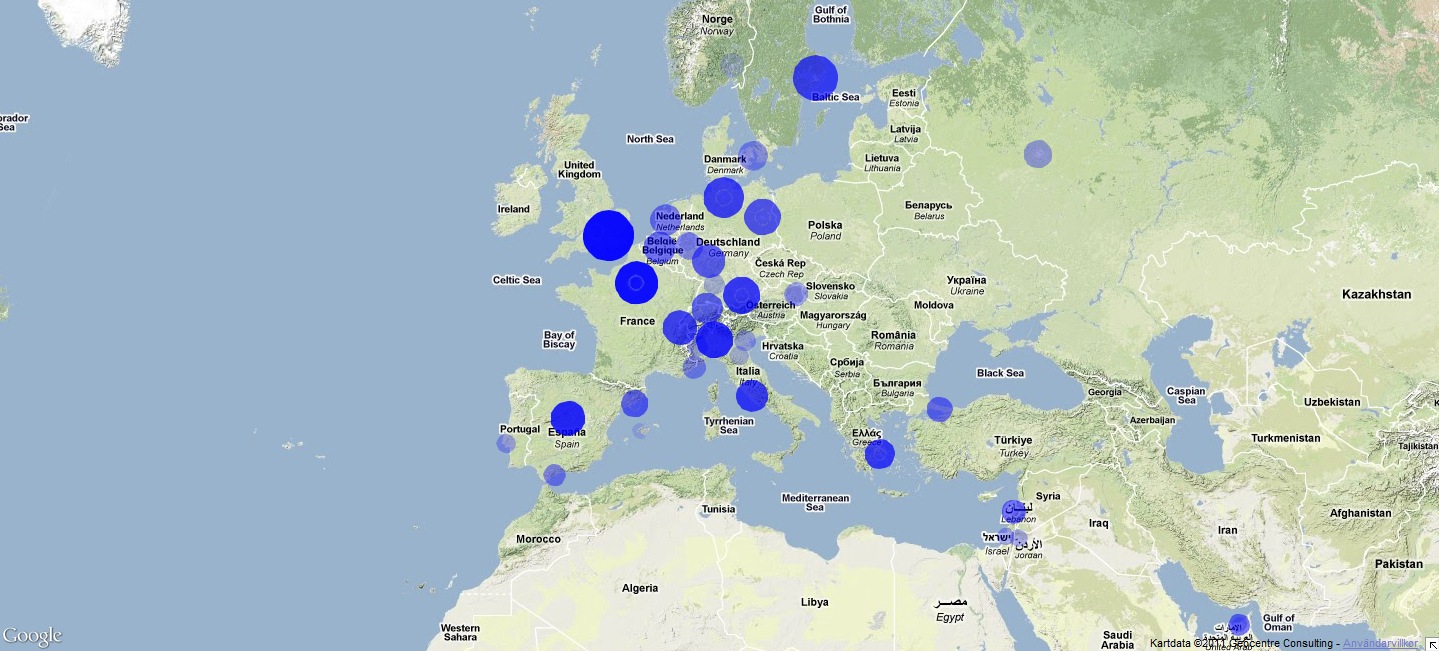
\includegraphics[width=130mm]{img/post-gordon}
							\end{center}
							\vspace{-13pt}
						\end{figure}	
						\bf interpretation: \rm not correlated
						\\ No difference between the week before and the week of election can be seen. This is probably due to the fact that there was a lot of press coverage and discussion already the week before his election. Therefore the forum activity is probably not related.
						
						
						
					\item \bf Chile Earthquake \rm
						\\ 8.0 Earthquake in Peru kills over 500 people, injures over 1,500; 7.7 Earthquake in northern Chile.
						\\\\ \bf time span: \rm August 15 - August 29
						\\ \bf geographical area: \rm South America
						\\ \bf total number of threads: \rm 3033
						\begin{figure}[H]
							\vspace{-13pt}
  							\begin{center}
								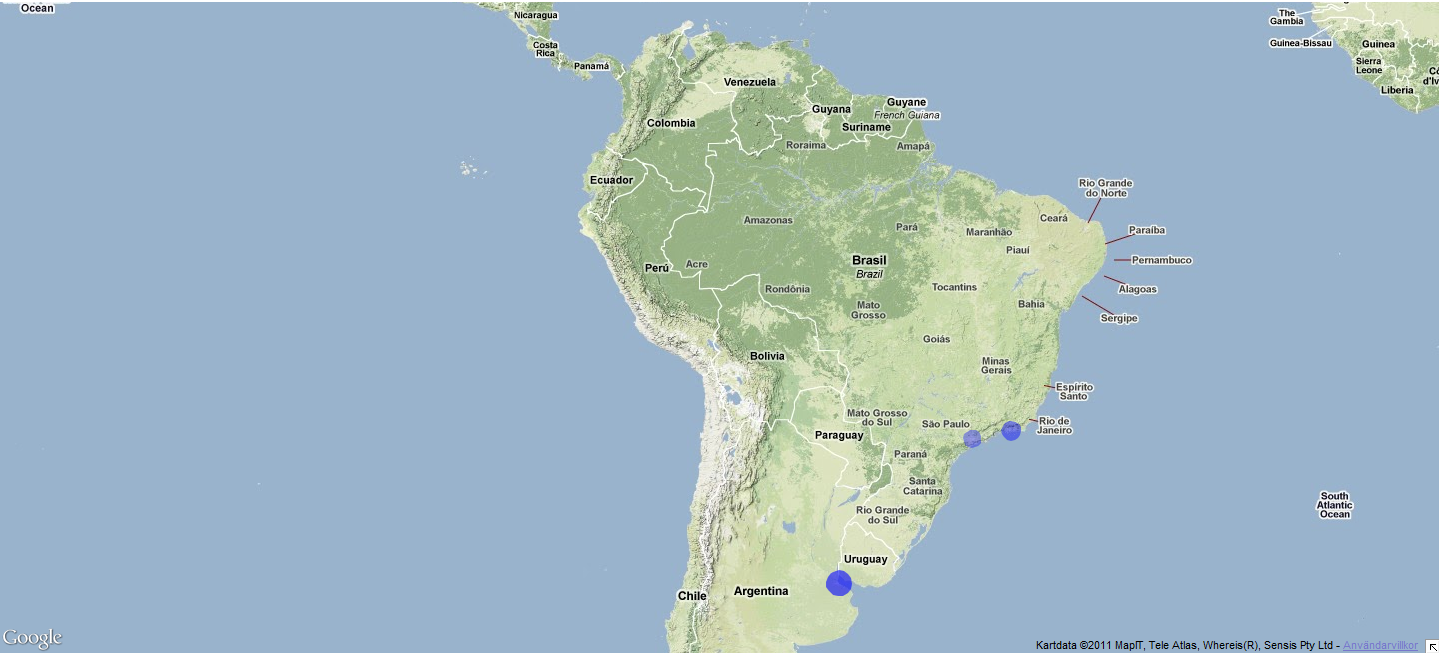
\includegraphics[width=130mm]{img/pre-chile}
							\end{center}
							\vspace{-13pt}
						\end{figure}
						\begin{figure}[H]
							\vspace{-13pt}
							\begin{center}
								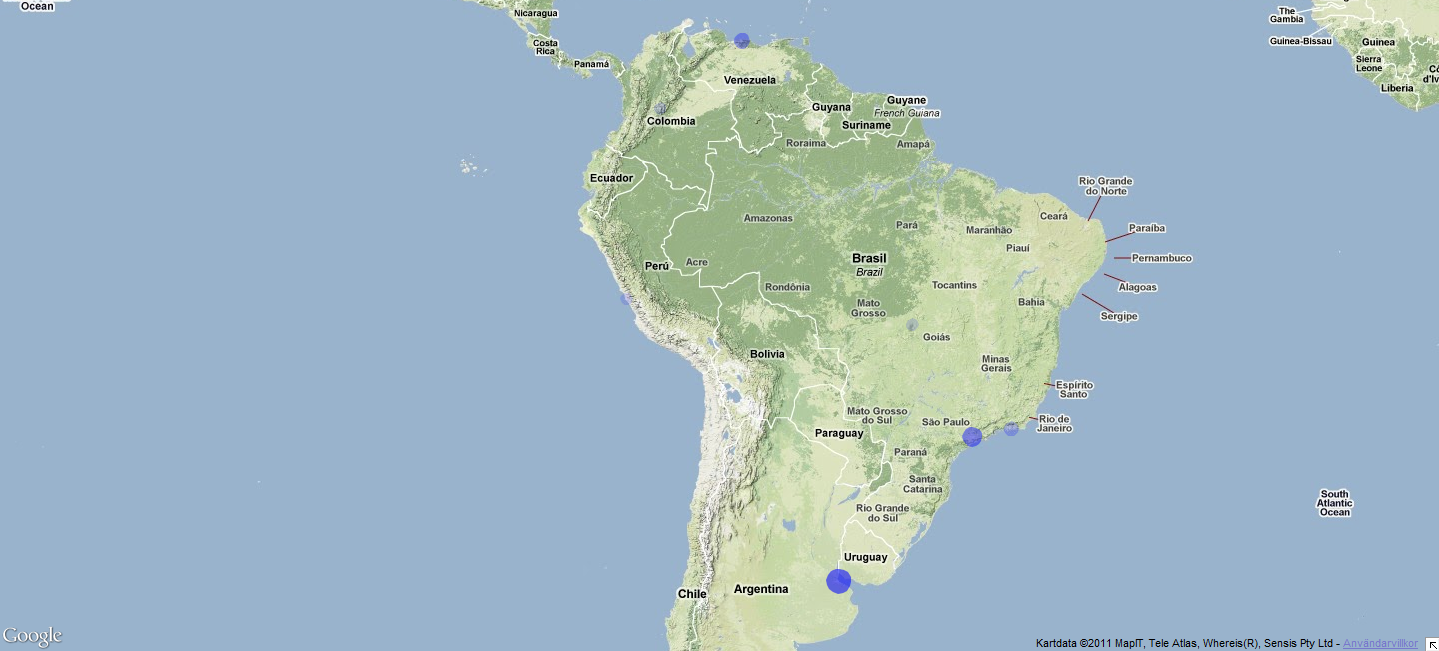
\includegraphics[width=130mm]{img/post-chile}
							\end{center}
							\vspace{-13pt}
						\end{figure}	
						\bf interpretation: \rm correlated
						\\ There's activity in south american cities that have never shown activity before - including cities in Venezuela, Columbia, Brasil, Peru and Chile. This is most probably correlated to the earthquakes in Chile.
						
						
						
					\item \bf Writers Guild goes on strike \rm
						\\ The Writers Guild of America goes on a strike that lasts until February 12, 2008. More than 12,000 writers joined the strike. The strike's goal was to rectify what was perceived as a historical injustice to America: the greatly diminished monetary compensation the writers got in comparison with the profits of the larger studios. The guilds were on strike 100 days.
						\\\\ \bf time span: \rm November - December
						\\ \bf geographical area: \rm Los Angeles, USA
						\\ \bf total number of threads: \rm 10234
						\begin{figure}[H]
							\vspace{-13pt}
  							\begin{center}
								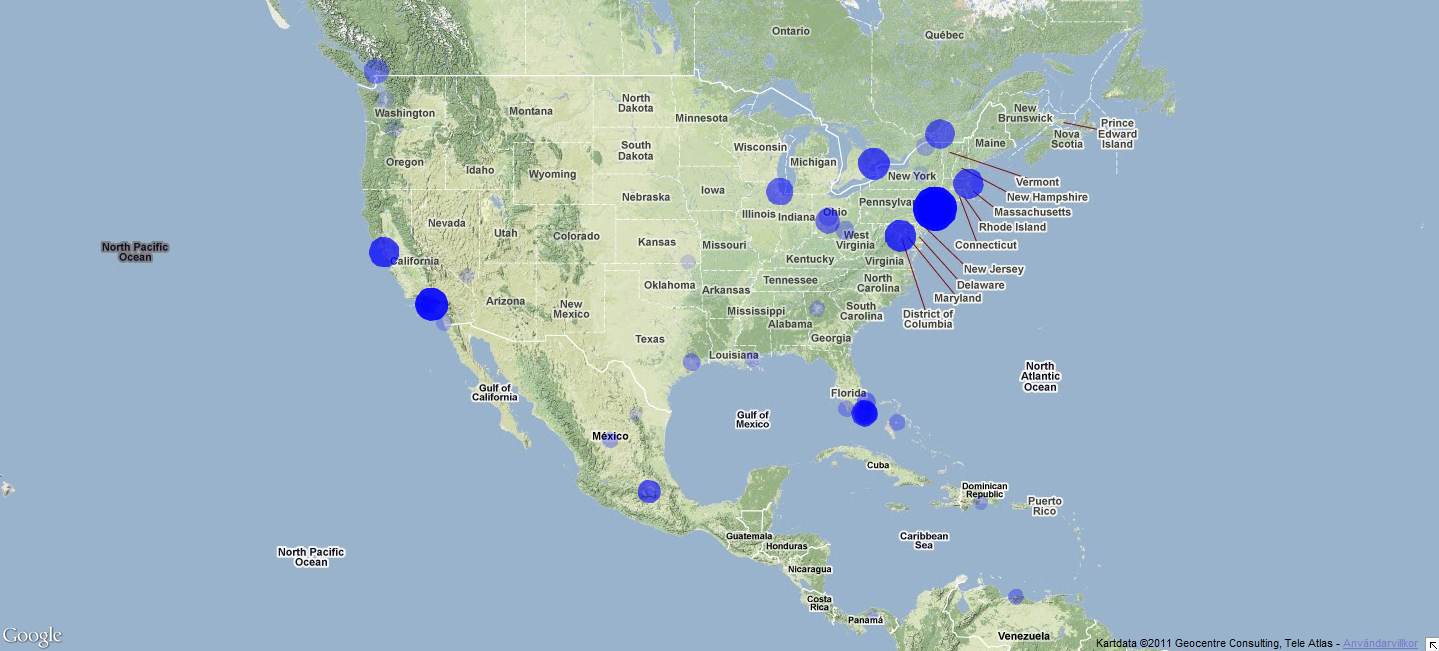
\includegraphics[width=130mm]{img/pre-writer}
							\end{center}
							\vspace{-13pt}
						\end{figure}
						\begin{figure}[H]
							\vspace{-13pt}
	  						\begin{center}
								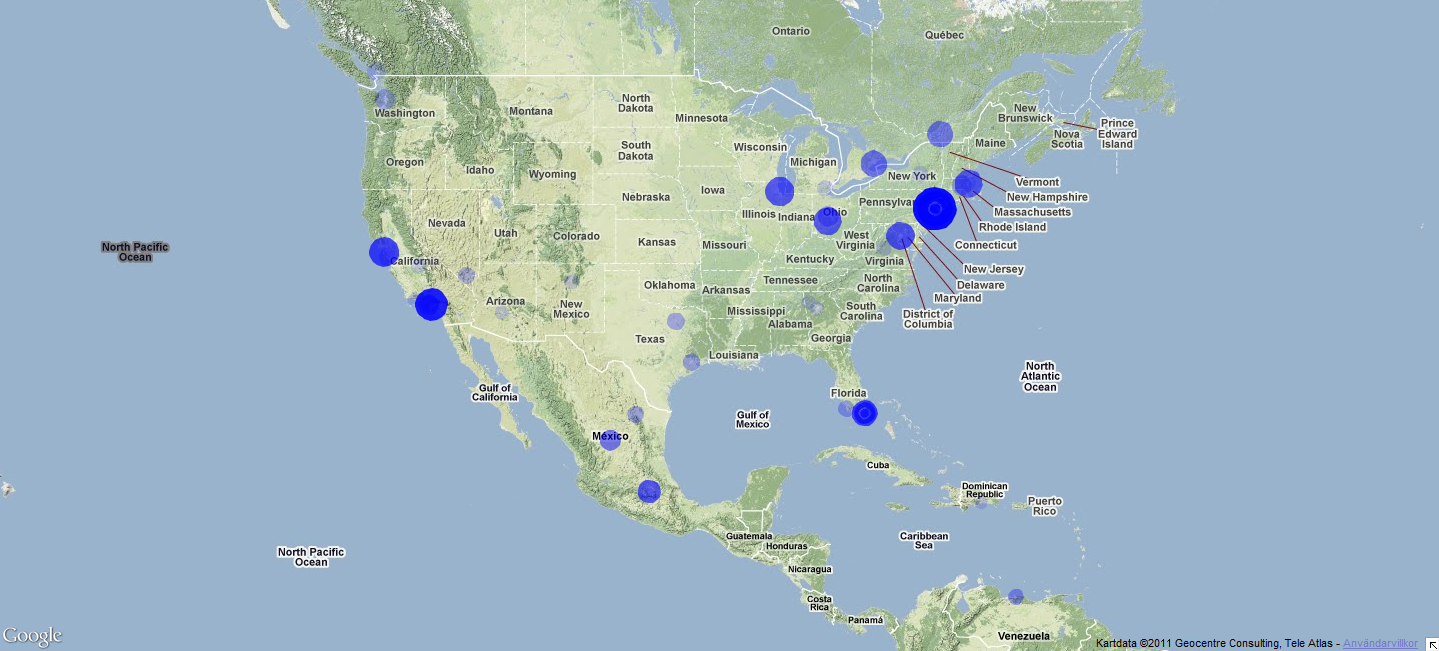
\includegraphics[width=130mm]{img/post-writer}
							\end{center}
							\vspace{-13pt}
						\end{figure}	
						\bf interpretation: \rm not correlated
						\\ There's not visual change of the activity during the strike. The Writers Guild's strike was probably not a often discussed topic on ASW and the activity is therefore not correlated.
						
						
						
				\end{itemize}
			
			\subsection{2008}
			\href{http://social.moldova.org/news/10-most-important-world-events-of-2008-217389-eng.html}{Top10 Events in 2008 on moldova.org}
				\begin{itemize}
					\item \bf Kosovo declares independency \rm
						\\ Kosovo declares independence from Serbia, announced by prime minister Hashim Thaci. Serbian prime minister Vojislav Kostunica says he would never recognize the "false state." International reaction is mixed, with the United States, France, Germany, and Britain indicating that they plan to recognize Kosovo as the world's 195th country.
						\\\\ \bf time span: \rm February 17 - March 17
						\\ \bf geographical area: \rm Kosovo
						\\ \bf total number of threads: \rm 5250
						\begin{figure}[H]
							\vspace{-13pt}
  							\begin{center}
								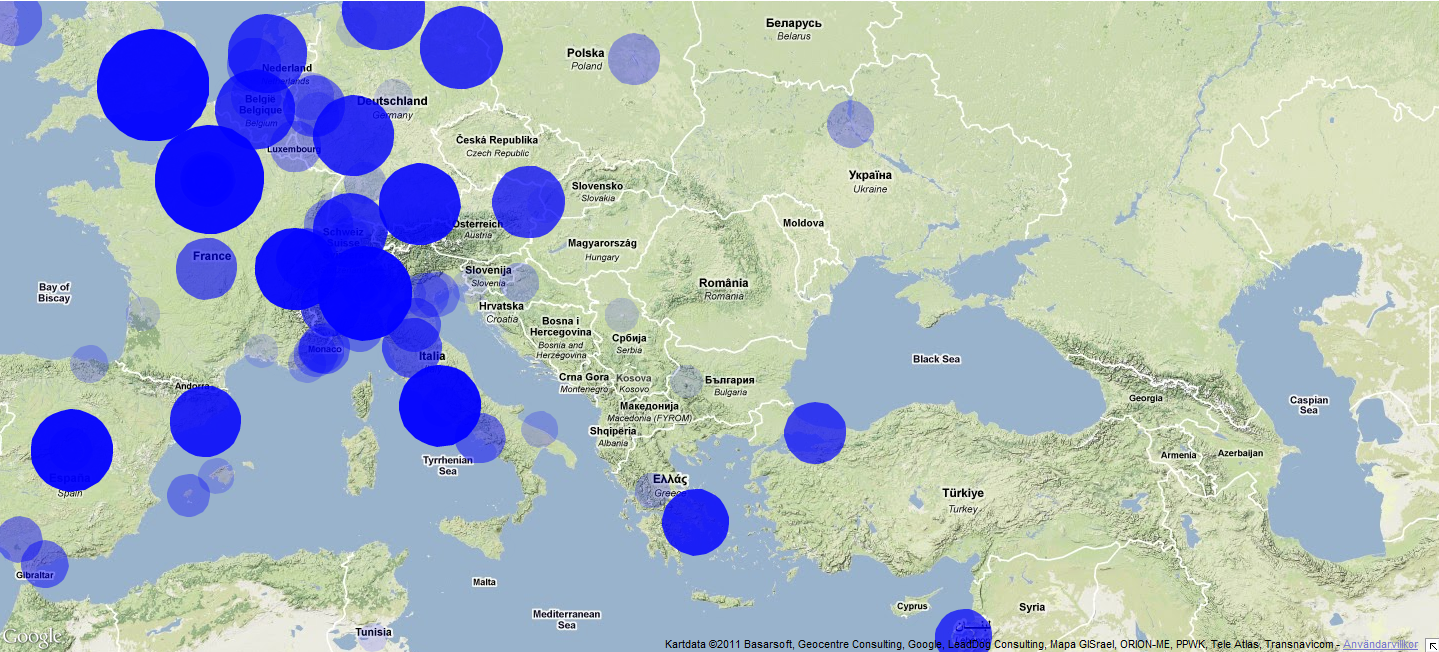
\includegraphics[width=130mm]{img/pre-kosovo}
							\end{center}
							\vspace{-13pt}
						\end{figure}
						\begin{figure}[H]
							\vspace{-13pt}
	  						\begin{center}
								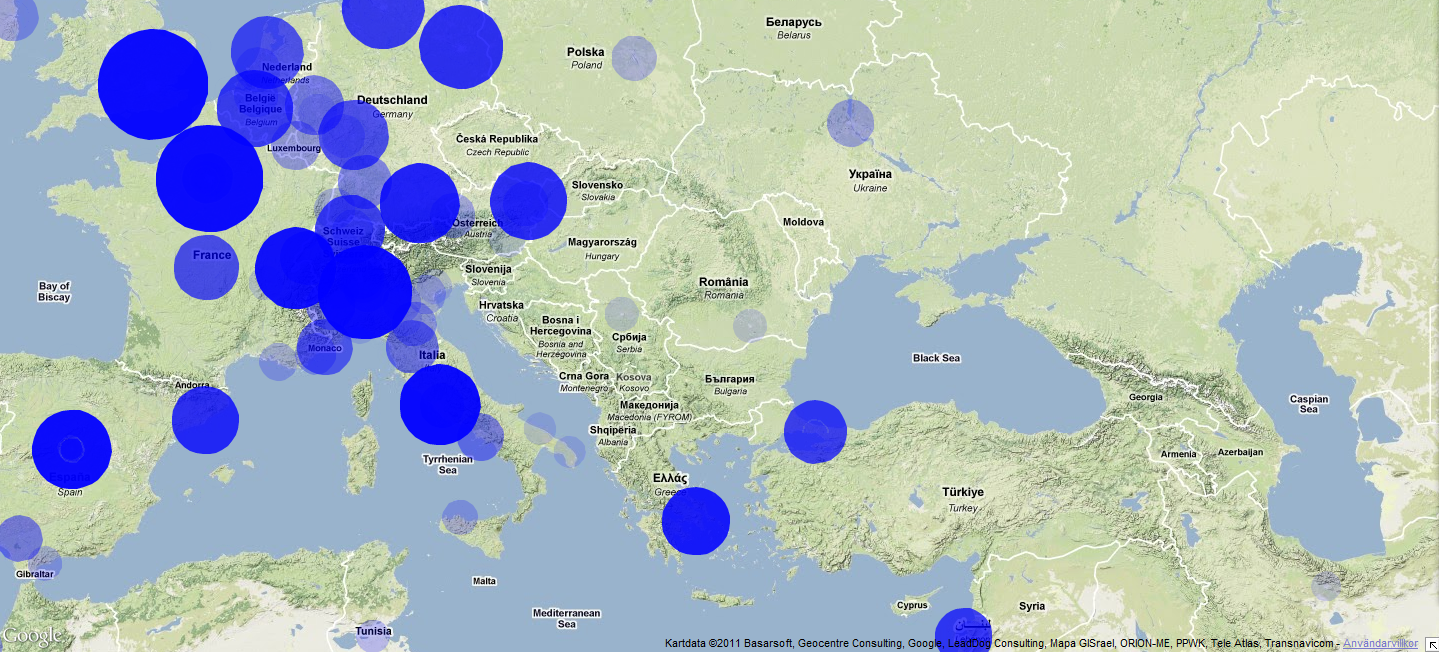
\includegraphics[width=130mm]{img/post-kosovo}
							\end{center}
							\vspace{-13pt}
						\end{figure}	
						\bf interpretation: \rm correlated
						\\ We found some activity in a city in Kosovo and increased activity in Kosovo's surroundings which makes us think that the forum activity and the happenings in Kosovo are related in this case.
						
						
						
					\item \bf Medvedev becomes Russia's President \rm
						\\ Russia in 2008 chooses another president - Dmitri A. Medvedev, a former aide to Russian president Vladimir Putin, wins the presidential election in a landslide. Putin will remain in a position of power, serving as Medvedev's prime minister.
						\\\\ \bf time span: \rm March 2 - March 9
						\\ \bf geographical area: \rm Russia
						\\ \bf total number of threads: \rm 1353
						\begin{figure}[H]
							\vspace{-13pt}
  							\begin{center}
								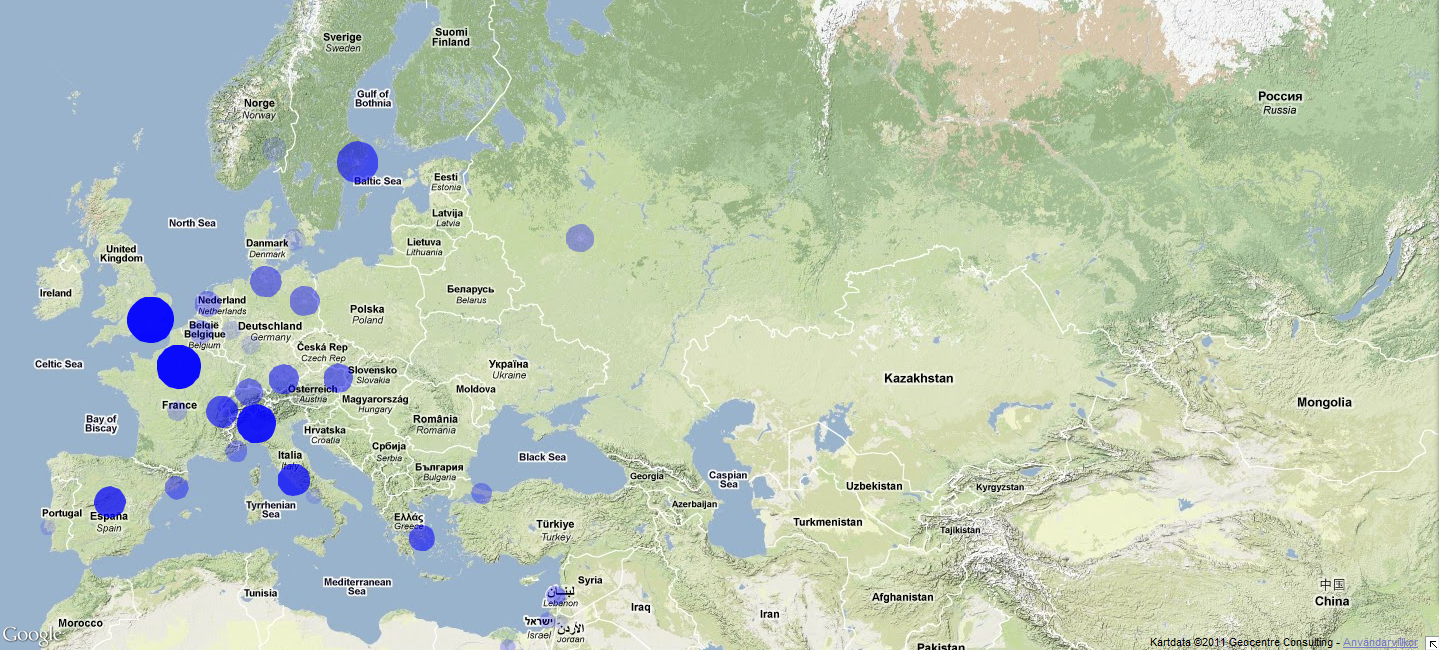
\includegraphics[width=130mm]{img/pre-medvev}		
							\end{center}
							\vspace{-13pt}
						\end{figure}
						\begin{figure}[H]
							\vspace{-13pt}
	  						\begin{center}
								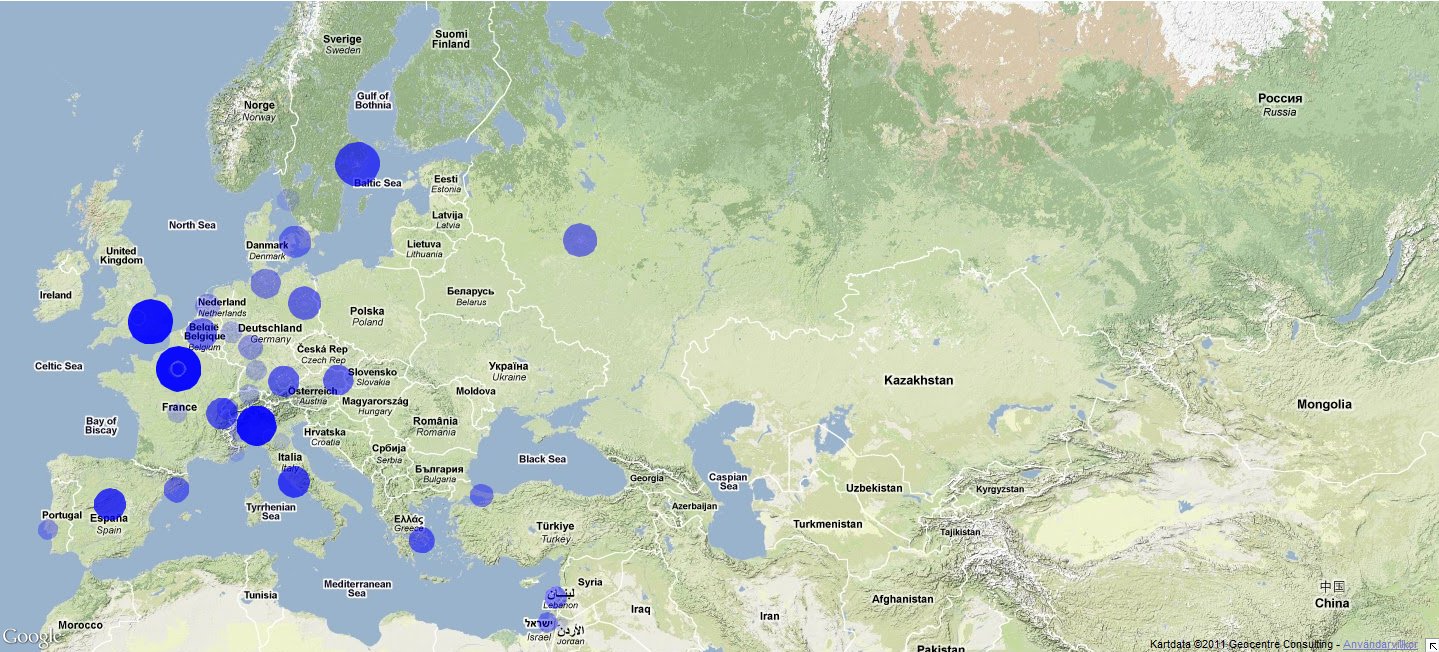
\includegraphics[width=130mm]{img/post-medvev}
							\end{center}
							\vspace{-13pt}
						\end{figure}	
						\bf interpretation: \rm not correlated
						\\ We could not see a big increase of activity in Russia or its neighborhood and we therefore think that the forum activity and this event are not correlated.

					
					
					\item \bf China's Earthquake \rm
						\\On May 12, 2008, a magnitude 7.9 earthquake struck the Sichuan Province of China, killing more than 69,000 people, making it China's worst disaster in more than 30 years.
						\\\\ \bf time span: \rm May 12 - May 26
						\\ \bf geographical area: \rm China
						\\ \bf total number of threads: \rm 1660
						\begin{figure}[H]
							\vspace{-13pt}
  							\begin{center}
								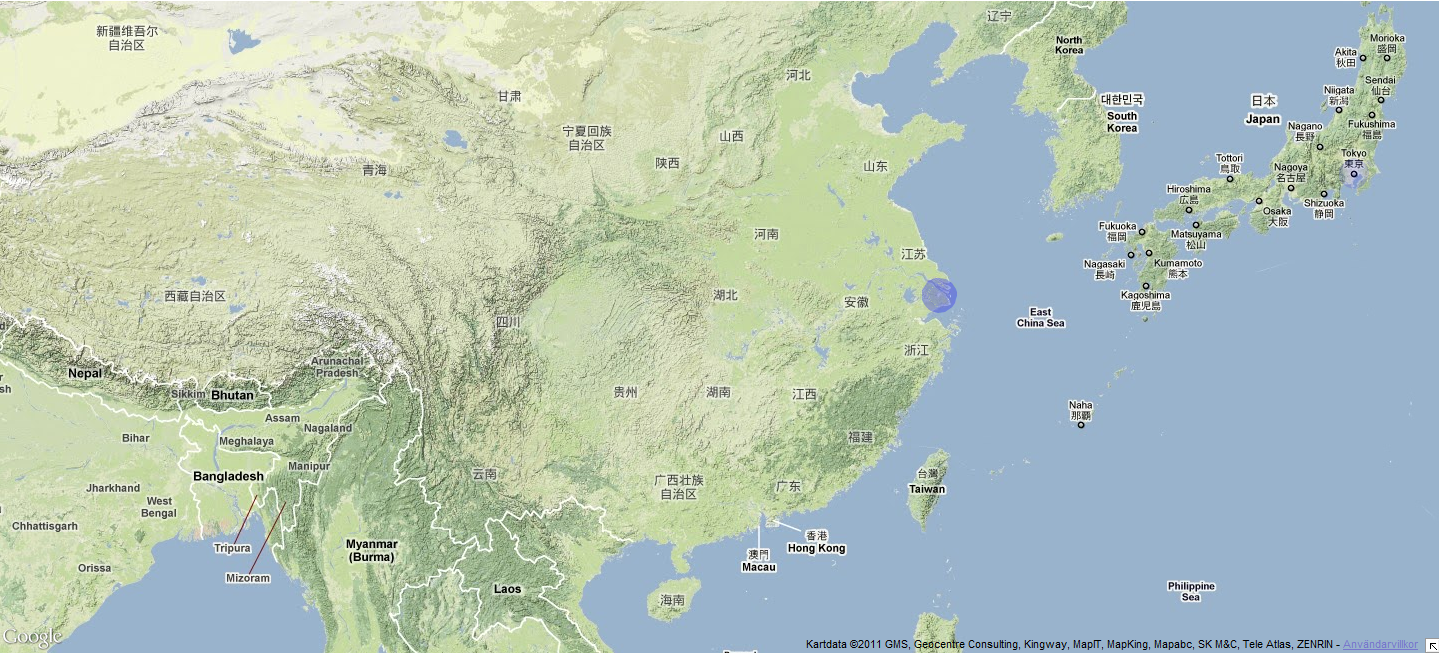
\includegraphics[width=130mm]{img/pre-china}
							\end{center}
							\vspace{-13pt}
						\end{figure}
						\begin{figure}[H]
							\vspace{-13pt}
	  						\begin{center}
								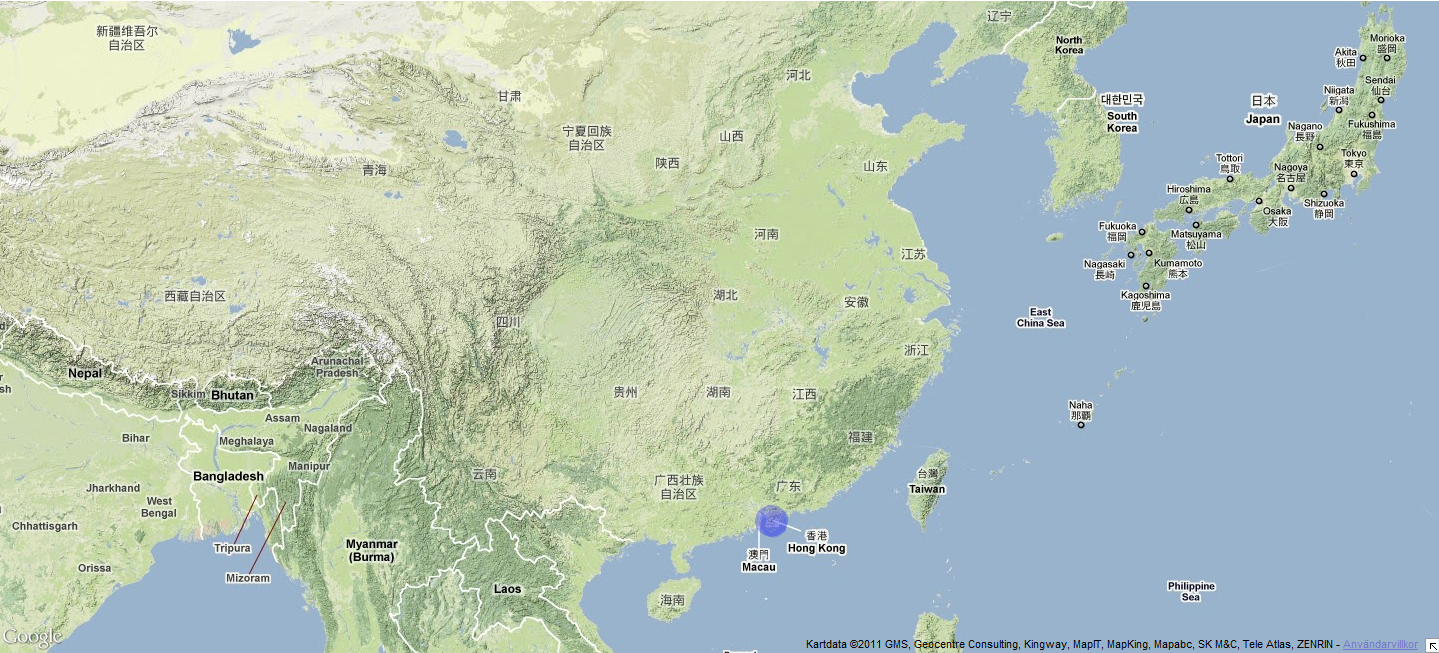
\includegraphics[width=130mm]{img/post-china}
							\end{center}
							\vspace{-13pt}
						\end{figure}						
						\bf interpretation: \rm not correlated
						\\ There's almost no activity in Asia during this period and therefore the forum activity was not related to the real world events.
						
						

					\item \bf Summer Olympic Games \rm
						\\ Summer Olympic Games 2008 that took place in Beijing, China. It was the XXIX Olympiad. The international multi-sport event officially opened on August 6 and ended on August 24, featuring 10,500 athletes who struggled for the Olympic Gold medal in 302 events in 28 sports. The Summer Olympic Games 2008 was really worth remembering, showing remarkable performances of the athletes: 43 new world records and 132 new Olympic records. Besides, representative of 87 countries won at least one medal at these Olympics, an unprecedented achievement.
						\\\\ \bf time span: \rm August 8 - 24
						\\ \bf geographical area: \rm Beijing, China
						\\ \bf total number of threads: \rm 1124
						\begin{figure}[H]
							\vspace{-13pt}
  							\begin{center}
								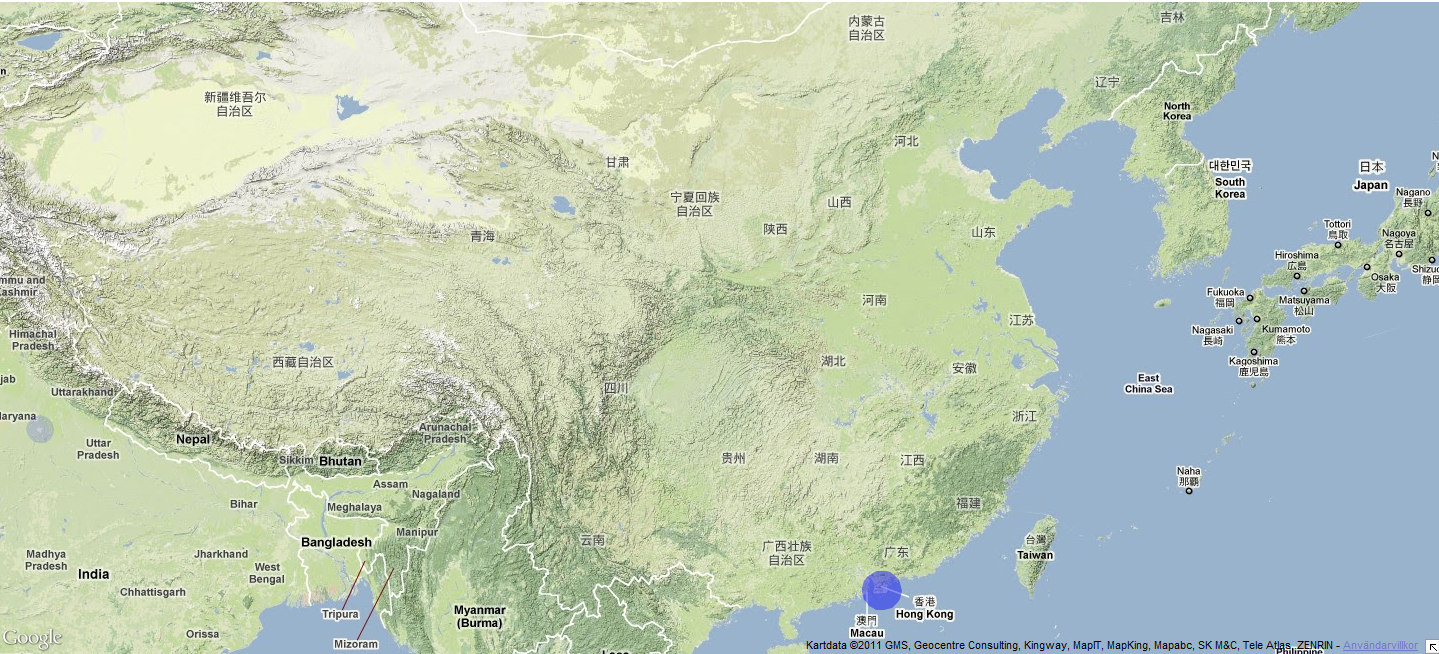
\includegraphics[width=130mm]{img/pre-olympic}
							\end{center}
							\vspace{-13pt}
						\end{figure}
						\begin{figure}[H]
							\vspace{-13pt}
	  						\begin{center}
								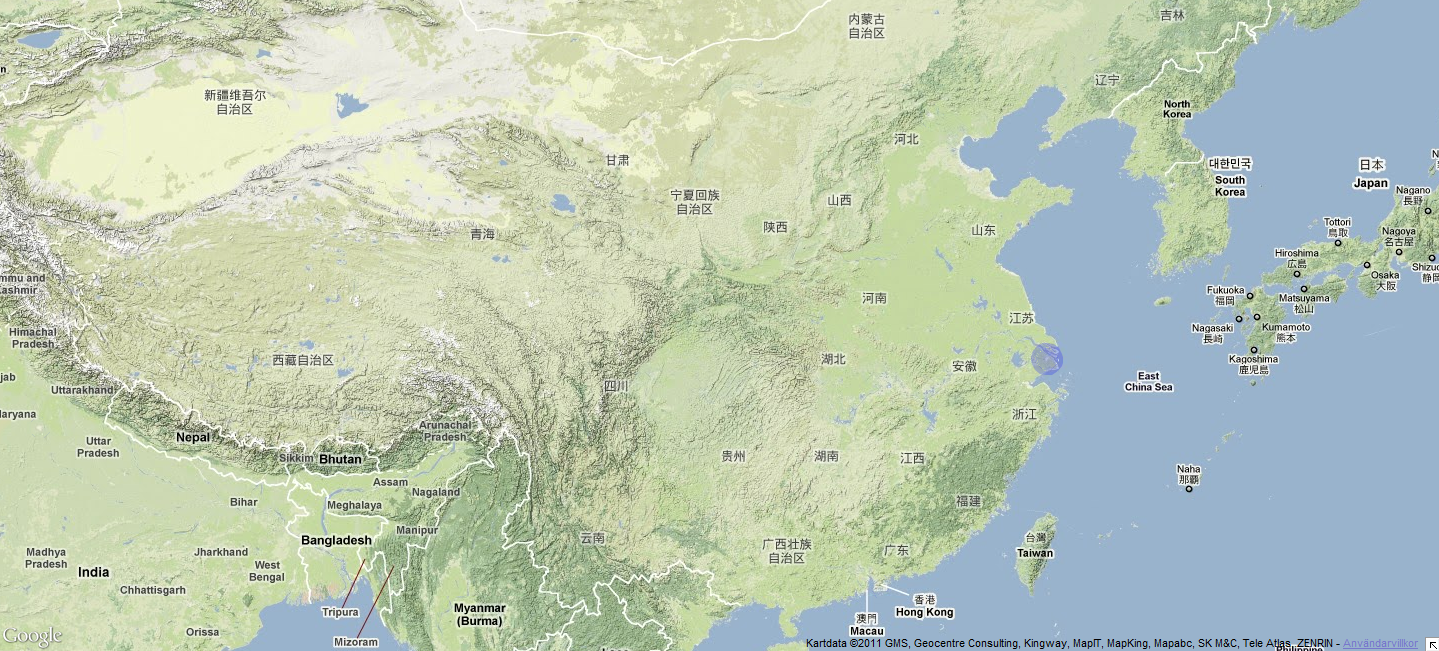
\includegraphics[width=130mm]{img/post-olympic}
							\end{center}
							\vspace{-13pt}
						\end{figure}	
						\bf interpretation: \rm not correlated
						\\ The only activity seen in china moved from Hong Kong to Shanghai during this period. Not correlated to what happens in Beijing at this time.
						
						
				\end{itemize}
			
			\subsection{2009}
			\href{http://social.moldova.org/news/10-most-important-world-events-of-2009-217390-eng.html}{Top10 Events in 2009 on moldova.org}
				\begin{itemize}
					\item \bf Swine Flu \rm
						\\ The "swine flu", the H1N1 influenza strain is the first condition deemed a global pandemic since the Hong Kong flu of 1967 to 1968. According to the latest WHO statistics, the virus has killed more than 18,000 people since it appeared in April 2009 and were 622,482 infected (approximate).
						\\\\ \bf time span: \rm November 1 2008 - February 31 2009
						\\ \bf geographical area: \rm global 
						\\ \bf total number of threads: \rm
						\begin{figure}[H]
							\vspace{-13pt}
  							\begin{center}
								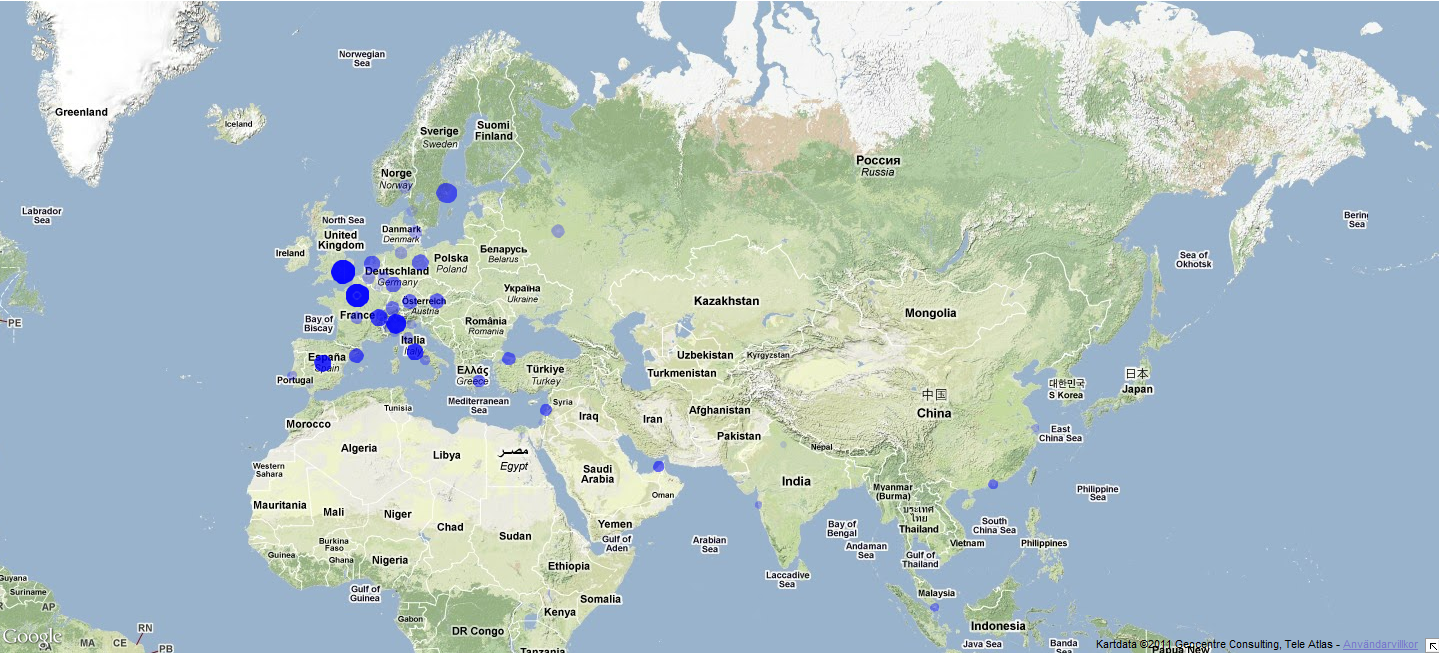
\includegraphics[width=130mm]{img/pre-birdflu}
							\end{center}
							\vspace{-13pt}
						\end{figure}
						\begin{figure}[H]
							\vspace{-13pt}
	  						\begin{center}
								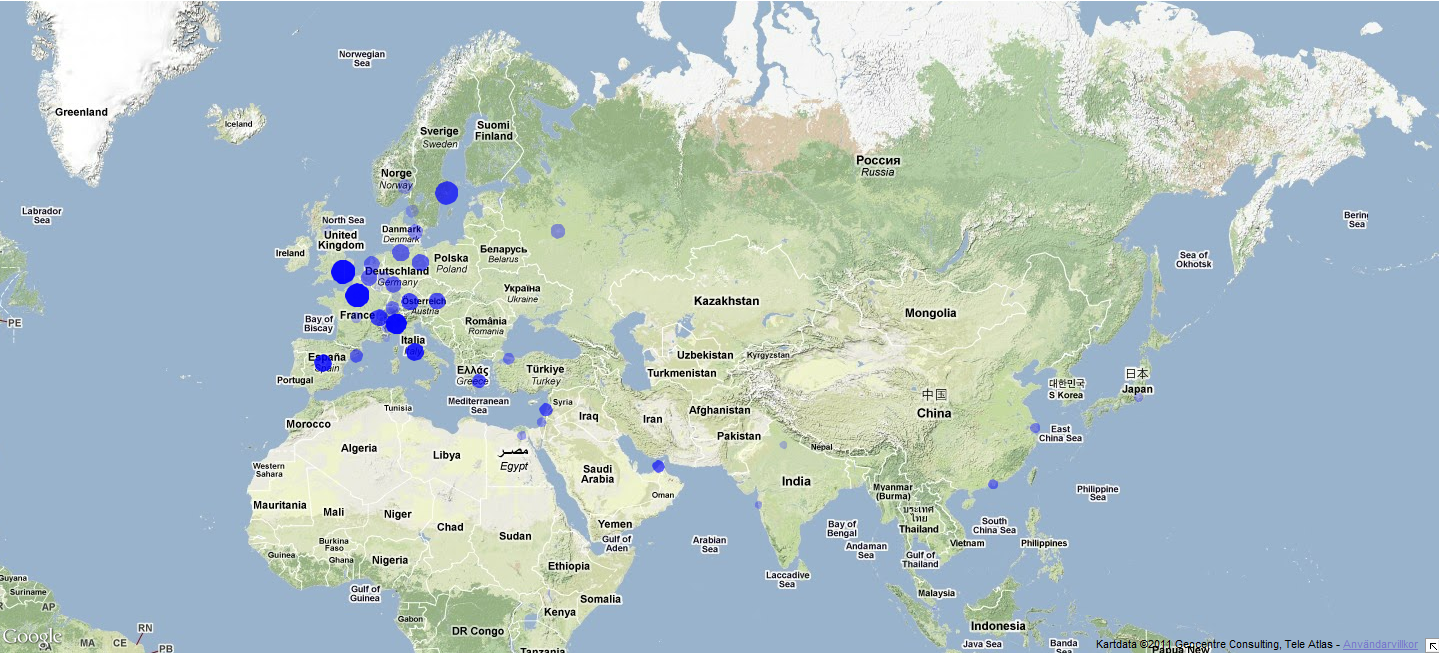
\includegraphics[width=130mm]{img/post-birdflu}
							\end{center}
							\vspace{-13pt}
						\end{figure}	
						\bf interpretation: \rm probably not correlated
						\\ We could not conclude whether the event and the forum activity were correlated as the time span is probably too big to make any distinction
						
						
					\item \bf Michael Jackson's death \rm
						\\ Michael Jackson the most famous US singer dies after he suffered cardiac arrest at his home in the Holmby Hills neighborhood in Los Angeles, California. Later the Los Angeles County Coroner declared Jackson's death a homicide caused by the combination of drugs in his body.
						\\ Conrad Murray is the doctor that had to take care of Michael's health before his death, and in 2011 he is still under charge of involuntary manslaughter. Internet traffic reaches unprecedented levels after entertainer Michael Jackson's death triggers an outpouring of worldwide grief.
						\\\\ \bf time span: \rm June 25 - July 2
						\\ \bf geographical area: \rm USA
						\\ \bf total number of threads: \rm 38724
						
						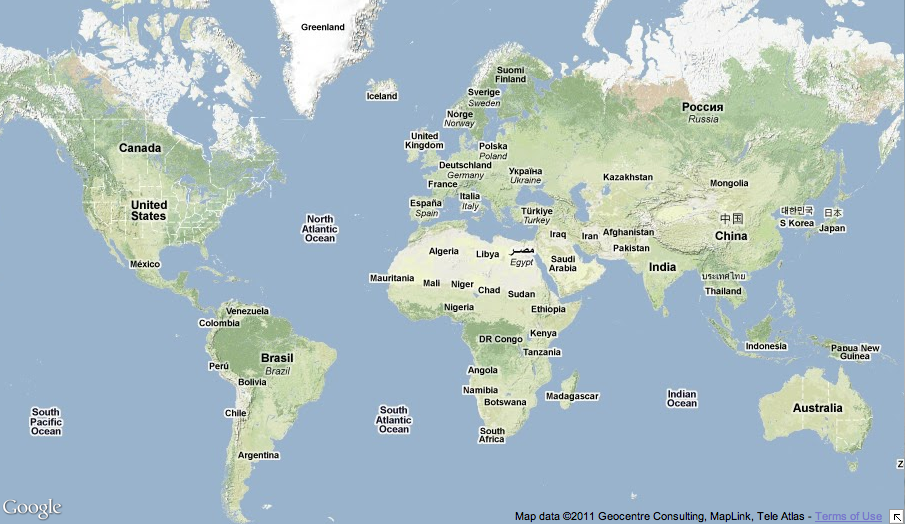
\includegraphics[width=130mm]{img/2005-1}
						
						\bf interpretation: \rm YES OR NO - ARE WE IMPRESSED? :)
						Basically the browser died during the second day because the enormous amount of circles on the map exceeded what memory we could use.
						
						
%					\item \bf Silvio Berlusconi attacked \rm
%						\\ Italian Prime Minister Silvio Burlusconi is knocked to the ground and hit in the face after a political rally in Milan, Italy. An attacker hurled a statuette at Italian Premier striking the leader in the face. The attacker is a 42-year-old Massimo Tartaglia, a graphic designer with a history of mental problems. The attack occurred at a difficult political time for Berlusconi, who has been plagued by scandals.
%						\\\\ \bf time span: \rm December 14 - December 28
%						\\ \bf geographical area: \rm Italy
%						\\ \bf total number of threads: \rm 0
%						
%						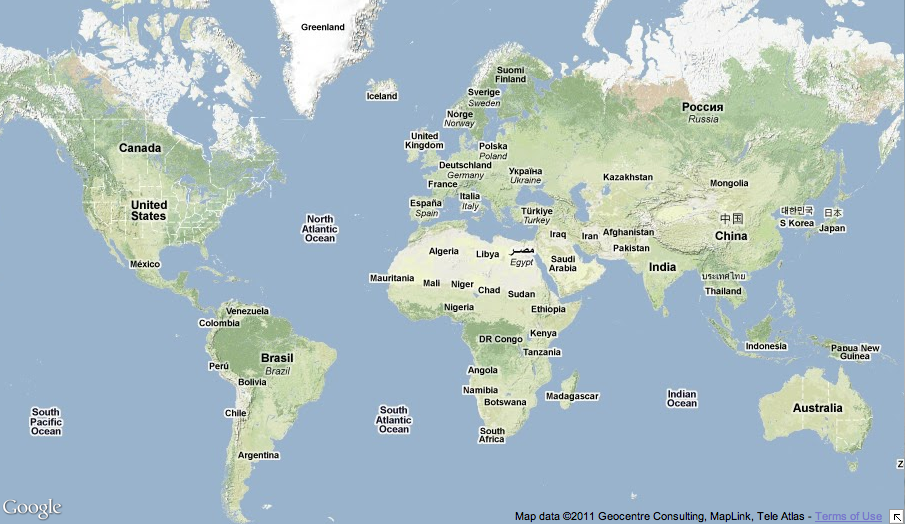
\includegraphics[width=130mm]{img/2005-1}
%						
%						\bf interpretation: \rm YES OR NO - ARE WE IMPRESSED? :)
						
					
						
				\end{itemize}
 \newpage	
	\section{Conclusion}
		The Visualizer built for our project is currently available at \url{http://cedricwaldburger.ch/comp621u/main.html} and will be removed by the end of the semester. 

		The code can be pulled from Github on this address \url{https://github.com/Hirschen/comp621u}.

\end{document}